\documentclass{article}
\usepackage{fullpage}
\usepackage{amsmath,amssymb,amsthm}
\usepackage[hidelinks]{hyperref}
\usepackage{graphicx}
\usepackage[utf8]{inputenc}
\usepackage{xcolor}
\usepackage{natbib}
% \usepackage{subcaption}
\usepackage{lineno}

\bibliographystyle{plainnat}

\newcommand{\comdist}{\widetilde{R}}
\newcommand{\comdistfn}{\widetilde{\mathcal{R}}}

\newcommand{\R}{\mathbb{R}}
\newcommand{\norm}[1]{\left\lVert#1\right\rVert}
\DeclareMathOperator{\var}{\mathop{\mbox{Var}}}
\DeclareMathOperator{\cov}{\mathop{\mbox{Cov}}}
\DeclareMathOperator{\diag}{\mathop{\mbox{diag}}}
\renewcommand{\P}{\mathbb{P}}
\newcommand{\E}{\mathbb{E}}
\newcommand{\given}{\,\vert\,}
\newcommand{\supp}{\mathop{\mbox{supp}}}
\newcommand{\sgn}{\mathop{\mbox{sgn}}}
\newcommand{\PP}[1]{\P\!\left\{#1\right\}}
\newcommand{\bone}{\mathbf{1}}

\newcommand{\plr}[1]{{\em \color{blue} #1}}

\newif\ifsubmission
% \submissiontrue  % for submission
\submissionfalse % for actual reading

%%% WARNING: right now, with submissiontrue, the supplemental figures dissappear
%%% and are not referred to!!
\ifsubmission
    % \renewcommand{\includegraphics}[2][]{\relax}
    \usepackage{endfloat}
    % \renewcommand{\efloatseparator}{\mbox{}} 
\fi

% Responses to reviews:
% set this to show line numbers and include responses to reviews or not
\newif\ifreviewresponses
\reviewresponsestrue  % include them
% \reviewresponsesfalse  % don't include them
\usepackage{lineno}
\usepackage{blindtext}
\usepackage{hyperref}


%%%%%  PUT THIS IN HEADER OF FILE
% % Responses to reviews:
% \usepackage{lineno}
\usepackage{blindtext}
\usepackage{hyperref}


%%%%%  PUT THIS IN HEADER OF FILE
% % Responses to reviews:
% \usepackage{lineno}
\usepackage{blindtext}
\usepackage{hyperref}


%%%%%  PUT THIS IN HEADER OF FILE
% % Responses to reviews:
% \input{review-response-commands}
% % set this to show line numbers and include responses to reviews or not
% \newif\ifreviewresponses
% \reviewresponsestrue  % include them
% % \reviewresponsesfalse  % don't include them
% \newcommand{\responsefile}{the-review-responses.tex}  % name of the review reponses file

\ifreviewresponses
\linenumbers
\else
\renewcommand{\linelabel}[1]{\relax}
\fi

% counters for reviewer points
\newcommand{\thereviewer}{}
\newcounter{point}
\setcounter{point}{0}

% pass in to \reviewersection the label for this reviewer (i.e. \reviewersection{1} or \reviewersection{AE})
\newcommand{\reviewersection}[1]{\renewcommand{\thereviewer}{#1}
                  \setcounter{point}{0}
                  \section*{Reviewer \thereviewer:}}
% drawing from from http://tex.stackexchange.com/questions/2317/latex-style-or-macro-for-detailed-response-to-referee-report
%% arguments to \point are (name of the point, optional) and (content)
\newenvironment{point}[1]
        { \refstepcounter{point} \bigskip \hrule \medskip \noindent 
                \slshape {\fontseries{b}\selectfont (\thereviewer.\thepoint) #1} }
        { }
\newcommand{\reply}{\normalfont \medskip \noindent \textbf{Reply}:\ }   

% Use this command in the text where a change addressing a reviewer point has occurred
% e.g. \revpoint{1}{3} for reviewer 1, point 3
\newcommand{\revpoint}[2]{\hypertarget{llineno:rr:rev#1:#2}{\linelabel{rr:rev#1:#2}}}
% and this one to refer to such a location, e.g. \revreffull{1}{3}
\newcommand{\revreffull}[2]{\hyperlink{llineno:rr:rev#1:#2}{(p.\ \pageref{rr:rev#1:#2}, l.\ \lineref{rr:rev#1:#2})}}
% but this version fills in reviewer and point automatically if called in the appropriate part of the reviews
\newcommand{\revref}{\revreffull{\thereviewer}{\thepoint}}
% NOTE: should call \revref{} with empty brackets after to get a space afterwards if desired: http://tex.stackexchange.com/questions/31091/space-after-latex-commands
% hyperlinks drawing from https://tex.stackexchange.com/questions/117883/hyperlinks-and-line-numbering

% Use this one to refer to a named linelabel
% e.g. if in the text there is a \llabel{approx_eqn_point}
% refer to it with \llname{approx_eqn_point}
\newcommand{\llabel}[1]{\hypertarget{llineno:#1}{\linelabel{#1}}}
\newcommand{\llname}[1]{\hyperlink{llineno:#1}{(p.\ \pageref{#1}, l.\ \lineref{#1})}}

% put \includereviews() where the reviews are to appear (at the end?)
\newcommand{\includereviews}{
    \ifreviewresponses
    \clearpage
    \setcounter{page}{1}
    \setcounter{section}{0}
    \setcounter{subsection}{0}
    \nolinenumbers
    % \begin{center}
    %   {\LARGE \bf Response to Reviews}
    % \end{center}
    \input{\responsefile}
    \fi
}

% Useful shortcuts ;) that demonstrate how to use the macros.
\newcommand{\rollover}{ \reply{The reviewer makes an excellent point that we have missed out entirely.  We have made all the changes suggested, down to the minutiae \revref.} }
\newcommand{\playdead}{ \reply{The reviewer makes an excellent point.  We have made an utterly trivial change {\revref} that we think deals entirely with the concern raised.} }
                                                                                                         
% from http://tex.stackexchange.com/questions/43648/why-doesnt-lineno-number-a-paragraph-when-it-is-followed-by-an-align-equation/55297#55297
\ifcsname{patchAmsMathEnvironmentForLineno}\endcsname
    \newcommand*\patchAmsMathEnvironmentForLineno[1]{%                                                       
      \expandafter\let\csname old#1\expandafter\endcsname\csname #1\endcsname                                
      \expandafter\let\csname oldend#1\expandafter\endcsname\csname end#1\endcsname                          
      \renewenvironment{#1}%                                                                                 
         {\linenomath\csname old#1\endcsname}%                                                               
         {\csname oldend#1\endcsname\endlinenomath}}%                                                        
    \newcommand*\patchBothAmsMathEnvironmentsForLineno[1]{%                                                  
      \patchAmsMathEnvironmentForLineno{#1}%                                                                 
      \patchAmsMathEnvironmentForLineno{#1*}}%                                                               
    \AtBeginDocument{%                                                                                       
    \patchBothAmsMathEnvironmentsForLineno{equation}%                                                        
    \patchBothAmsMathEnvironmentsForLineno{align}%                                                           
    \patchBothAmsMathEnvironmentsForLineno{flalign}%                                                         
    \patchBothAmsMathEnvironmentsForLineno{alignat}%                                                         
    \patchBothAmsMathEnvironmentsForLineno{gather}%                                                          
    \patchBothAmsMathEnvironmentsForLineno{multline}%                                                        
\fi

% % set this to show line numbers and include responses to reviews or not
% \newif\ifreviewresponses
% \reviewresponsestrue  % include them
% % \reviewresponsesfalse  % don't include them
% \newcommand{\responsefile}{the-review-responses.tex}  % name of the review reponses file

\ifreviewresponses
\linenumbers
\else
\renewcommand{\linelabel}[1]{\relax}
\fi

% counters for reviewer points
\newcommand{\thereviewer}{}
\newcounter{point}
\setcounter{point}{0}

% pass in to \reviewersection the label for this reviewer (i.e. \reviewersection{1} or \reviewersection{AE})
\newcommand{\reviewersection}[1]{\renewcommand{\thereviewer}{#1}
                  \setcounter{point}{0}
                  \section*{Reviewer \thereviewer:}}
% drawing from from http://tex.stackexchange.com/questions/2317/latex-style-or-macro-for-detailed-response-to-referee-report
%% arguments to \point are (name of the point, optional) and (content)
\newenvironment{point}[1]
        { \refstepcounter{point} \bigskip \hrule \medskip \noindent 
                \slshape {\fontseries{b}\selectfont (\thereviewer.\thepoint) #1} }
        { }
\newcommand{\reply}{\normalfont \medskip \noindent \textbf{Reply}:\ }   

% Use this command in the text where a change addressing a reviewer point has occurred
% e.g. \revpoint{1}{3} for reviewer 1, point 3
\newcommand{\revpoint}[2]{\hypertarget{llineno:rr:rev#1:#2}{\linelabel{rr:rev#1:#2}}}
% and this one to refer to such a location, e.g. \revreffull{1}{3}
\newcommand{\revreffull}[2]{\hyperlink{llineno:rr:rev#1:#2}{(p.\ \pageref{rr:rev#1:#2}, l.\ \lineref{rr:rev#1:#2})}}
% but this version fills in reviewer and point automatically if called in the appropriate part of the reviews
\newcommand{\revref}{\revreffull{\thereviewer}{\thepoint}}
% NOTE: should call \revref{} with empty brackets after to get a space afterwards if desired: http://tex.stackexchange.com/questions/31091/space-after-latex-commands
% hyperlinks drawing from https://tex.stackexchange.com/questions/117883/hyperlinks-and-line-numbering

% Use this one to refer to a named linelabel
% e.g. if in the text there is a \llabel{approx_eqn_point}
% refer to it with \llname{approx_eqn_point}
\newcommand{\llabel}[1]{\hypertarget{llineno:#1}{\linelabel{#1}}}
\newcommand{\llname}[1]{\hyperlink{llineno:#1}{(p.\ \pageref{#1}, l.\ \lineref{#1})}}

% put \includereviews() where the reviews are to appear (at the end?)
\newcommand{\includereviews}{
    \ifreviewresponses
    \clearpage
    \setcounter{page}{1}
    \setcounter{section}{0}
    \setcounter{subsection}{0}
    \nolinenumbers
    % \begin{center}
    %   {\LARGE \bf Response to Reviews}
    % \end{center}
    \input{\responsefile}
    \fi
}

% Useful shortcuts ;) that demonstrate how to use the macros.
\newcommand{\rollover}{ \reply{The reviewer makes an excellent point that we have missed out entirely.  We have made all the changes suggested, down to the minutiae \revref.} }
\newcommand{\playdead}{ \reply{The reviewer makes an excellent point.  We have made an utterly trivial change {\revref} that we think deals entirely with the concern raised.} }
                                                                                                         
% from http://tex.stackexchange.com/questions/43648/why-doesnt-lineno-number-a-paragraph-when-it-is-followed-by-an-align-equation/55297#55297
\ifcsname{patchAmsMathEnvironmentForLineno}\endcsname
    \newcommand*\patchAmsMathEnvironmentForLineno[1]{%                                                       
      \expandafter\let\csname old#1\expandafter\endcsname\csname #1\endcsname                                
      \expandafter\let\csname oldend#1\expandafter\endcsname\csname end#1\endcsname                          
      \renewenvironment{#1}%                                                                                 
         {\linenomath\csname old#1\endcsname}%                                                               
         {\csname oldend#1\endcsname\endlinenomath}}%                                                        
    \newcommand*\patchBothAmsMathEnvironmentsForLineno[1]{%                                                  
      \patchAmsMathEnvironmentForLineno{#1}%                                                                 
      \patchAmsMathEnvironmentForLineno{#1*}}%                                                               
    \AtBeginDocument{%                                                                                       
    \patchBothAmsMathEnvironmentsForLineno{equation}%                                                        
    \patchBothAmsMathEnvironmentsForLineno{align}%                                                           
    \patchBothAmsMathEnvironmentsForLineno{flalign}%                                                         
    \patchBothAmsMathEnvironmentsForLineno{alignat}%                                                         
    \patchBothAmsMathEnvironmentsForLineno{gather}%                                                          
    \patchBothAmsMathEnvironmentsForLineno{multline}%                                                        
\fi

% % set this to show line numbers and include responses to reviews or not
% \newif\ifreviewresponses
% \reviewresponsestrue  % include them
% % \reviewresponsesfalse  % don't include them
% \newcommand{\responsefile}{the-review-responses.tex}  % name of the review reponses file

\ifreviewresponses
\linenumbers
\else
\renewcommand{\linelabel}[1]{\relax}
\fi

% counters for reviewer points
\newcommand{\thereviewer}{}
\newcounter{point}
\setcounter{point}{0}

% pass in to \reviewersection the label for this reviewer (i.e. \reviewersection{1} or \reviewersection{AE})
\newcommand{\reviewersection}[1]{\renewcommand{\thereviewer}{#1}
                  \setcounter{point}{0}
                  \section*{Reviewer \thereviewer:}}
% drawing from from http://tex.stackexchange.com/questions/2317/latex-style-or-macro-for-detailed-response-to-referee-report
%% arguments to \point are (name of the point, optional) and (content)
\newenvironment{point}[1]
        { \refstepcounter{point} \bigskip \hrule \medskip \noindent 
                \slshape {\fontseries{b}\selectfont (\thereviewer.\thepoint) #1} }
        { }
\newcommand{\reply}{\normalfont \medskip \noindent \textbf{Reply}:\ }   

% Use this command in the text where a change addressing a reviewer point has occurred
% e.g. \revpoint{1}{3} for reviewer 1, point 3
\newcommand{\revpoint}[2]{\hypertarget{llineno:rr:rev#1:#2}{\linelabel{rr:rev#1:#2}}}
% and this one to refer to such a location, e.g. \revreffull{1}{3}
\newcommand{\revreffull}[2]{\hyperlink{llineno:rr:rev#1:#2}{(p.\ \pageref{rr:rev#1:#2}, l.\ \lineref{rr:rev#1:#2})}}
% but this version fills in reviewer and point automatically if called in the appropriate part of the reviews
\newcommand{\revref}{\revreffull{\thereviewer}{\thepoint}}
% NOTE: should call \revref{} with empty brackets after to get a space afterwards if desired: http://tex.stackexchange.com/questions/31091/space-after-latex-commands
% hyperlinks drawing from https://tex.stackexchange.com/questions/117883/hyperlinks-and-line-numbering

% Use this one to refer to a named linelabel
% e.g. if in the text there is a \llabel{approx_eqn_point}
% refer to it with \llname{approx_eqn_point}
\newcommand{\llabel}[1]{\hypertarget{llineno:#1}{\linelabel{#1}}}
\newcommand{\llname}[1]{\hyperlink{llineno:#1}{(p.\ \pageref{#1}, l.\ \lineref{#1})}}

% put \includereviews() where the reviews are to appear (at the end?)
\newcommand{\includereviews}{
    \ifreviewresponses
    \clearpage
    \setcounter{page}{1}
    \setcounter{section}{0}
    \setcounter{subsection}{0}
    \nolinenumbers
    % \begin{center}
    %   {\LARGE \bf Response to Reviews}
    % \end{center}
    \input{\responsefile}
    \fi
}

% Useful shortcuts ;) that demonstrate how to use the macros.
\newcommand{\rollover}{ \reply{The reviewer makes an excellent point that we have missed out entirely.  We have made all the changes suggested, down to the minutiae \revref.} }
\newcommand{\playdead}{ \reply{The reviewer makes an excellent point.  We have made an utterly trivial change {\revref} that we think deals entirely with the concern raised.} }
                                                                                                         
% from http://tex.stackexchange.com/questions/43648/why-doesnt-lineno-number-a-paragraph-when-it-is-followed-by-an-align-equation/55297#55297
\ifcsname{patchAmsMathEnvironmentForLineno}\endcsname
    \newcommand*\patchAmsMathEnvironmentForLineno[1]{%                                                       
      \expandafter\let\csname old#1\expandafter\endcsname\csname #1\endcsname                                
      \expandafter\let\csname oldend#1\expandafter\endcsname\csname end#1\endcsname                          
      \renewenvironment{#1}%                                                                                 
         {\linenomath\csname old#1\endcsname}%                                                               
         {\csname oldend#1\endcsname\endlinenomath}}%                                                        
    \newcommand*\patchBothAmsMathEnvironmentsForLineno[1]{%                                                  
      \patchAmsMathEnvironmentForLineno{#1}%                                                                 
      \patchAmsMathEnvironmentForLineno{#1*}}%                                                               
    \AtBeginDocument{%                                                                                       
    \patchBothAmsMathEnvironmentsForLineno{equation}%                                                        
    \patchBothAmsMathEnvironmentsForLineno{align}%                                                           
    \patchBothAmsMathEnvironmentsForLineno{flalign}%                                                         
    \patchBothAmsMathEnvironmentsForLineno{alignat}%                                                         
    \patchBothAmsMathEnvironmentsForLineno{gather}%                                                          
    \patchBothAmsMathEnvironmentsForLineno{multline}%                                                        
\fi

\newcommand{\responsefile}{review-responses.tex}  % name of the review reponses file

\newcommand*\patchAmsMathEnvironmentForLineno[1]{%
  \expandafter\let\csname old#1\expandafter\endcsname\csname #1\endcsname
  \expandafter\let\csname oldend#1\expandafter\endcsname\csname end#1\endcsname
  \renewenvironment{#1}%
     {\linenomath\csname old#1\endcsname}%
     {\csname oldend#1\endcsname\endlinenomath}}% 
\newcommand*\patchBothAmsMathEnvironmentsForLineno[1]{%
  \patchAmsMathEnvironmentForLineno{#1}%
  \patchAmsMathEnvironmentForLineno{#1*}}%
\AtBeginDocument{%
\patchBothAmsMathEnvironmentsForLineno{equation}%
\patchBothAmsMathEnvironmentsForLineno{align}%
\patchBothAmsMathEnvironmentsForLineno{flalign}%
\patchBothAmsMathEnvironmentsForLineno{alignat}%
\patchBothAmsMathEnvironmentsForLineno{gather}%
\patchBothAmsMathEnvironmentsForLineno{multline}%
}

\begin{document}

\title{Are populations like a circuit? 
Comparing isolation by resistance to a new coalescent-based method.}
\author{Erik Lundgren\footnote{Computational Biology, University of Southern California}, and
        Peter L.\ Ralph\footnote{Institute for Ecology and Evolution, University of Oregon}}
\maketitle

\linenumbers

\begin{abstract}
A number of methods commonly used in landscape genetics
use an analogy to electrical resistance on a network
to describe and fit barriers to movement across the landscape
using genetic distance data.
These are motivated by a mathematical equivalence between electrical resistance 
between two nodes of a network
and the ``commute time'',
which is the mean time for a random walk on that network to leave one node, visit the other, and return.
However, genetic data are more accurately modeled by a different quantity,
the coalescence time.
Here, we describe the differences between resistance distance and coalescence time,
and explore the consequences for inference.
We implement a Bayesian method to infer effective movement rates and population sizes 
under both these models,
and find that inference using commute times
can produce misleading results in the presence of biased gene flow.
We then use forwards-time simulation with continuous geography to demonstrate that
coalescence-based inference remains more accurate than resistance-based methods on realistic data,
but difficulties highlight the need for methods 
that explicitly model continuous, heterogeneous geography.
\end{abstract}


%%%%%%%%%%%%%%%%%%%%%%
\section*{Introduction}

Genetic relatedness is determined by past gene flow,
a product of individual or gamete movements across geographic space.
Genomes therefore retain the traces of this movement,
and can contribute to the inference of how a species moves across a landscape,
which is important for understanding how diseases spread, how species adapt,
and how to retain genetic diversity in threatened species.
This is a potentially important source of information,
as direct observation can be difficult 
(especially of long-distance movement, \citep{cayuelademographic,levin_et_al_seed_dispersal}),
or even impossible, if some of the populations in question no longer exist. \revpoint{3}{18}

The idea of ``resistance distance'' is an important tool in the landscape genomics toolbox.
Introduced by \citet{mcrae2006isolation},
it makes use of a mathematical equivalence between random walks and electrical resistance
\citep{nashwilliams1959random}:
the expected time for a continuous-time Markov chain that starts at node $x$
to first hit node $y$ and then return to $x$ (the ``commute time'')
is equal to the effective resistance between $x$ and $y$ in an electrical network
whose conductances are given by the movement rates of the Markov chain \citep{levin2008markov,doyle2006random}.
This measure therefore averages over all possible paths through the network between the two.
Suppose we
assign local conductances based on the values of some landscape variable, 
and compute the correlation of
genetic distances between samples from different parts of the landscape
with the effective resistances between the samples' locations.
\revpoint{4}{2}
If this results in a significant positive correlation,
then this is taken as good evidence that the landscape variable is a good indicator of
where gene flow occurs \citep{mcrae2007circuit,cushman2006complex}.
For instance,
if the conductance across a grid cell in a discretization of the landscape
is higher in flatter areas,
and this produces effective resistance values 
that are significantly correlated with genetic distances,
then one might conclude that the species in question tends to disperse more readily through flatter areas,
perhaps along river valleys.
More recent methods \citep{petkova2016visualizing,hanks2013circuit} seek to build \emph{de novo} 
a map of conductance values that produces resistances 
most strongly correlated with observed genetic distance,
and then interpret regions of low conductance in the resulting map as barriers to gene flow.

As motivated by \citet{mcrae2006isolation},
commute time (i.e., resistance distance) is a computationally tractable approximation
to the more accurate random walk-based model of genetic distance,
the \emph{coalescence time}.
Genetic distances between two genomes sampled from the landscape
do derive from an average across a large number of paths between those points --
the lineages along which each segment of genetic material has been inherited
from their most recent common ancestor.
Thanks to recombination, there are a large number of such paths, 
and genetic distance averages over these.
The more recent these common ancestors tend to be,
the smaller the genetic distance is.
It is reasonable in some situations to model these lineages as random walks across the landscape;
however, the model of genetic distance that one is thus led to
is \emph{coalescence time} of the random walks, 
rather than commute time, the quantity that corresponds to resistance.
This naturally raises the question: 
Are methods that depend on effective resistances being misled by model misspecification?
If so, would using coalescence time do better?

\citet{mcrae2006isolation} showed that coalescence time and resistance distance are equal
(up to shift and scaling) in isotropic landscapes such as a ring \citep{matsen2006convergence},
and found that the two were highly correlated in several test cases.
However, all test cases had symmetric migration
(the same rate of gene flow in both directions along each edge),
which is likely not the case in many situations, e.g.,
in rivers \citep{morrissey2009maintenance,sundqvist2016directional,hanks2017modeling},
with source-sink dynamics \citep{dias1996sources},
or after population expansions \citep{with2002landscape}.

In this paper, we contrast 
coalescence time and resistance distance,
and develop a method to infer movement rates on a discrete landscape
using genetic distances.
As we will see,
although the two methods are conceptually similar,
resistance-based inference may infer movement rates uncorrelated with the truth \revpoint{3}{19}
if data are derived from a coalescent process,
especially in the presence of gene flow asymmetry. 
We also explore the question of identifiability.
Resistance-based methods are often used to predict distances based on a few layers of geographical data
(land cover, slope, etcetera).
Some methods find the combination of landscape layers to best explain genetic distance,
which allows very fine geographic resolution \citep{shaffer2017desert}.
Other methods such as EEMS \citep[``Estimating Effective Migration Surfaces'',][]{petkova2016visualizing} infer conductances without such prior information; \revpoint{3}{20}
however, the geographical resolution is much coarser.
(A recently-released method 
that is based on EEMS but uses haplotype length data and an underlying model of coalescence time
\citep{alasadi2018estimating}
is promising, but still produces similarly coarse maps.)
One reason for this difference in resolution
is that EEMS uses more computationally intensive Bayesian methods.
However, we show that this coarse resolution reflects a more general problem, \revpoint{3}{21}
both because of unmodeled ``process noise'' involved in discretization of geographical populations,
and the mathematical structure of the underlying problem.


%%%%%%%%%%%%%%%%%%
\section*{Methods}


The \emph{commute time} of a Markov chain between locations $i$ and $j$
is the expected time for a particle that moves according to the rules of the chain, 
started at $i$, to first reach $j$ and then return.
We will denote this by $R_{ij}$, to emphasize that it is also the effective resistance
between $i$ and $j$.
The \emph{coalescence time} is the expected time for two particles started at $i$ and $j$
to \emph{coalesce},
which happens at a given rate whenever they are in the same location.
We will denote this by $C_{ij}$.
Why should these be related to genetic distance? 
First, we explain this connection,
and then discuss their computation,
and finally develop a method that infers movement rates of the Markov chain
(which are reverse-time migration probabilities)
from observations of coalescence time, \revpoint{1}{9}
and apply this to a real dataset.
Although we have tried to highlight the intuitive aspects of this initial technical discussion,
readers who are interested in practical differences
more than the mathematical arguments should be able to skip to ``Test cases and simulations''
without loss of continuity. \llabel{ll:flagging}


%%%%%%%%%%%%%%%%%%%%%%%%%%%%%%%%%%%%%%%%%%%%%%%%%%%
\subsection*{Genetic distance and coalescence time}

There are a number of ways to calculate measures of dissimilarity using genetic data.
In this paper we use mean pairwise divergence, \revpoint{3}{6}
which for two genomes is calculated as the proportion of sites in the genome
at which the two genomes differ. \revpoint{3}{22}
It is more common in the literature to use $F_{ST}/(1-F_{ST})$, \revpoint{1}{7}
but the two are highly correlated for good theoretical reasons 
\citep{slatkin1991inbreeding,rousset1997genetic},
especially for SNP data.
(However, note that $F_{ST}$ depends on the sampling scheme, while divergence does not.) \revpoint{1}{7}
The two genomes differ at a site only if there has been a mutation in some ancestor on the lineages leading
from the two genomes back to their most recent common ancestor at that site.
Therefore,
under an infinite-sites model with average mutation rate $\mu$ per site and per meiosis,
pairwise divergence divided by $\mu$
is an unbiased estimate of the mean time to most recent common ancestor,
averaged across the genome \citep{hudson2007variance,ralph2015empirical}.
It is natural to model this process by following the two lineages back through time
(and across space)
until they find their most recent common ancestor,
i.e., until they coalesce.
Suppose we model the geographic distribution of the species
as a collection of randomly mating populations
that exchange occasional migrants,
thus discretizing geographic space.
It is common to assume that
the motion of these lineages back through time
forms a Markov process, the \emph{structured coalescent} \citep{wakeley2005coalescent}.
(This assumption requires the effects of natural selection on each segment of the genome 
to be generally weak.) \revpoint{3}{1}
In this framework, each lineage performs a random walk across the populations,
with movement probabilities depending on the flux of individuals between populations.
This provides the link between genetic distance and random walks.

For data, we are given genotypes of individuals and their geographic coordinates;
then, we divide these individuals into groups,
and compute the genetic distance between group $i$ and group $j$
as the mean divergence between a pair of genomes, chosen one from each group.
We denote the resulting genetic distance $D_{ij}$;
since divergence is symmetric, $D_{ij} = D_{ji}$.
We compute $D_{ii}$ by sampling without replacement from group $i$,
so that generally $D_{ii} > 0$: the diagonal elements measure local diversity.
As discussed below, we will find commute times so that the mean commute time between
$i$ and $j$ matches $D_{ij}$ -- but the commute time of a location to itself is zero,
so we must account for local diversity.
We do this in the same way as \citet{petkova2016visualizing},
by introducing the \emph{local diversity} parameters $q_i$,
and using the model
\begin{align} \label{eq:commute_approx}
	D_{ij} \approx \comdist_{ij} = R_{ij}/4 + q_{i}/2 + q_{j}/2 .
\end{align}
Concretely, this means finding 
movement rates of a Markov chain whose matrix of commute times ($R$)
yields a good approximation to the matrix of genetic distances,
after adding local diversity parameters ($q$, which are also free parameters). \revpoint{3}{7}
The factor of four is necessary to make commute time work on the same time scale as coalescence time:
the commute time covers the path from $i$ to $j$ twice
(once in both directions),
while the coalescence time covers the distance only once,
and in half the time, because two particles are moving.
% Furthermore, coalescence time includes within-location diversity
% because particles do not coalesce instantly --
% therefore, commute time is most analogous to the first meeting time.
For a conceptual picture of the differences between the coalescence time and commute time,
see Figure \ref{fig:concept_coalcom}. 

A simple situation when the two clearly differ \llabel{ll:threepop}
is in the presence of biased gene flow,
as for instance between a source and a sink population:
coalescence only requires that lineages move in \emph{one} direction
between populations,
while a commute requires movement in both.

\begin{figure}
\centering
     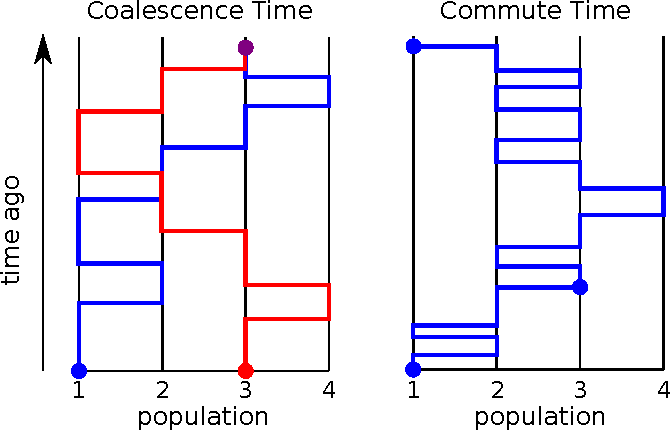
\includegraphics[scale=.5]{figs/conceptn}
    \caption{
    Illustration of the conceptual differences
    between coalescence and commute time between states 1 and 3 
    for a continuous time Markov chain with four linearly connected states. 
    Coalescence time (left) is the time for two independently moving particles to meet and coalesce 
    (it is possible for them to be in the same location without coalescing).
    Commute time is time for a single particle starting in one state to travel to another state 
    and then back to the original state.
    Note how the time axis is scaled to be faster in the figure showing commute time
    than the one for coalescence time in order for them to fit in the same space.
    } \label{fig:concept_coalcom}
\end{figure}


%%%%%%%%%%%%%%%%%%%%%%%%%%%%%%%%%%%%%%%%%%%%
\subsection*{Hitting times of Markov chains}

Now, we explain how to compute the relevant quantities --
mean commute and coalescence times -- from a Markov chain model of lineage movement.
The Markov chain is defined by its \emph{generator matrix}, denoted $G$,
for which $G_{xy}$ gives the ``jump rate'' from $x$ to $y$.
The jump rate $G_{xy}$ is \revpoint{3}{8}
the probability the chain jumps to position $y$ when at position $x$ per unit of time.
(More precisely, if the Markov chain is at location $X_t$ at time $t$,  \revpoint{5}{1}
then for $x \neq y$, $\PP{X_{t+\epsilon} = y \given X_t = x} = \epsilon G_{xy} + O(\epsilon^2)$.)
For mathematical convenience, the diagonal of this matrix is completed so that rows sum to zero:
$G_{xx} = - \sum_{y \neq x} G_{xy}$.
We will need to find the \emph{hitting times} of the chain --
i.e., for each pair of states $x$ and $y$, 
the mean time until the chain first hits $y$ after being started at $x$.
We denote this quantity $H_{xy}$.
Throughout, we assume that all hitting times are finite,
which implies the chain is connected and irreducible.
The Markov property lets us write a system of linear equations that can be solved for $H$, as follows
(see, e.g., \citet{kemeny1983finite}):
Suppose that the chain begins at $x \neq z$,
and is at location $y \neq z$ after $dt$ units of time, without having visited $z$.
Then the total time to hit $z$ is equal to the elapsed time $dt$
plus the remaining time to hit $z$ from $y$.
Formally, this says that \revpoint{5}{2}
$H_{xz} \approx dt + \sum_y \P\{X_{dt} = y \given X_0 = x\} H_{yz}$.
Replacing $\P\{X_{dt} = y \given X_0 = x\}$ with $dt G_{xy}$ and rearranging
gives the system of equations:
\begin{align} \label{eqn:hitting_sum}
    \sum_y G_{xy} H_{yz} = -1 \qquad \text{for} \; x \neq z.
\end{align}
In other words, if $G_{-z}$ is the matrix with the $z^\text{th}$ row and column removed,
and $\bone$ is the vector composed of all ones,
then the $z^\text{th}$ column of $H$, except for $H_{zz}$,
can be computed as $- (G_{-z})^{-1} \bone$.
This, along with $H_{zz} = 0$, allows computation of $H$
from the movement rates $G$ \citep{kemeny1983finite}.

Suppose instead we are given the hitting times, $H$, and wish to find the movement rates, $G$.
This is not the situation we are in -- we have either commute or coalescence times --
but it is related.
The Random Target Lemma \citep{aldous-fill-2014}
tells us that the stationary distribution of the Markov chain, denoted $\pi$,
can be recovered from the hitting times by solving $\pi = H^{-1} \bone / \bone^T H^{-1} \bone$.
As shown in Appendix \ref{apx::hitting_calcs},
equation \eqref{eqn:hitting_sum} can be rewritten in matrix form as
\begin{align} \label{eqn:gh}
    G H = \diag(1/\pi) - \bone \bone^T ,
\end{align}
which implies that $G$ can be computed directly from $H$ as
\begin{align} \label{eqn:G_from_H}
    G = \left( \diag(1/\pi) - \bone \bone^T \right) H^{-1} .
\end{align}
(We prove that $H$ is invertible in Appendix~\ref{apx::hitting_calcs}.) \revpoint{1}{12}
Therefore, $H$ uniquely determines $G$.

% \paragraph{Commute times}
The \emph{commute times} are a symmetrized version of the hitting times
(which need not be symmetric),
defining $R = H + H^T$, i.e.:
\begin{align} \label{eqn:R_from_H}
\text{\bf (commute time)} \qquad
    R_{xy} = H_{xy} + H_{yx}.
\end{align}

Although commute times are uniquely determined by movement rates, the reverse is not true --
we can use equations \eqref{eqn:gh} and \eqref{eqn:R_from_H} to see how to modify movement rates
without changing commute times.  \llabel{ll:dense1}
A small concrete example of this is given in Appendix \ref{ss:simple_example}.
More generally, commute times only depend on the symmetric part of $H$ --
given a skew-symmetric matrix $Z$ (so that $Z + Z^T = 0$),
any Markov chain that has hitting times given by $H_\epsilon = H + \epsilon Z$ for some $\epsilon$
will have the same commute times.
The resulting hitting times may not be valid --
if $G_\epsilon$ is the matrix constructed by applying equation \eqref{eqn:G_from_H} to $H_\epsilon$,
% (assuming this is invertible),
then it is not guaranteed that the offdiagonal elements of $G_\epsilon$ are all nonnegative, as required.
% (It is always true that rows of $G_\epsilon$ sum to zero.)
However, since $G$ and $H$ are continuous functions of each other,
if all offdiagonal elements of $G$ are strictly positive,
then there exists a positive $\epsilon_0$ such that all $G_\epsilon$ for $\epsilon < \epsilon_0$
do define valid Markov chains, all with the same commute times.

% \paragraph{Coalescence times}
The \emph{coalescence times} are defined using \emph{two} copies of the same chain,
as the mean time until coalescence,
if the chains coalesce at rate $\gamma$ when they are in the same place.
Concretely, 
suppose that $X$ and $Y$ are independent Markov chains both moving with movement rates given by $G$,
that coalesce at rate $\gamma_x$ when $X$ and $Y$ are both at $x$.
Then we define $\tau$ to be this coalescence time,
so that 
$\P\{\tau \le t + \epsilon \given \tau > t, \; X_t = Y_t = x\} = \epsilon \gamma_x + O(\epsilon^2)$,
and 
$\P\{\tau \le t + \epsilon \given \tau > t, \; X_t \neq Y_t\} = O(\epsilon^2)$.
Then, the (mean) coalescence time is $C_{xy} = \E[\tau \given X_0 = x, \, Y_0 = y]$.
A similar argument using the Markov property
shows that $C$ satisfies the following equation:
\begin{align}
\text{\bf (coalescence time)} \qquad
    \sum_y \left(G_{xy} C_{yz} + C_{xy} G_{zy}\right)
    &=
    \begin{cases}
        -1                   \quad & \text{if} \; x \neq z, \\
        -1 + \gamma_z C_{zz} \quad & \text{if} \; x = z.
    \end{cases}
\end{align}
Similar recursions are common in the literature,
going back at least to \citet{hill1972effective} (see also \citet{whitlock1997effective}).
In matrix notation, this is
\begin{align} \label{eqn:C_matrix}
    G C + C G^T - \diag(\gamma) \circ C = -\bone \bone^T,
\end{align}
where $\diag(\gamma)$ is the matrix with the vector $\gamma$ on the diagonal and zeros elsewhere,
and $\circ$ is the componentwise product.
In practice, we solve this by working with the product Markov chain $(X_t, Y_t)$,
whose generator matrix is $G \otimes I + I \otimes G$, \revpoint{1}{10}
where $I$ is the identity matrix and $\otimes$ is the Kronecker product.

Equation \eqref{eqn:C_matrix} is linear in $G$ and $\gamma$,
and so after rearrangement can be solved with standard linear algebra
(and is related to the Sylvester equation \citep{bhatia1997solve}).
However, the solution is again not necessarily unique:
suppose that we have a matrix $Z$ such that $ZC$ is skew-symmetric.
Then $(G + Z) C + C (G + Z)^T = GC + CG^T$,
and so a Markov chain with generator matrix $G + Z$ has the same coalescence times
as the original chain.
For $G + Z$ to be a valid generator, the rows of $Z$ must sum to zero,
and all offdiagonal entries of $G + Z$ must be nonnegative. \revpoint{1}{11}
As before, if all entries of $G$ are nonzero, 
it is always possible to find sufficiently small $\epsilon$
so that $G + \epsilon Z$ remains the generator of a valid Markov chain.

\paragraph{Constraints and uniqueness}
We have seen that to find the movement rates of a continuous-time Markov chain
given the coalescence or commute times
we must solve either equation \eqref{eqn:C_matrix} 
or equations \eqref{eqn:G_from_H} and \eqref{eqn:R_from_H} for $G$,
and that these do not have unique solutions.
The situation is worse when one needs to infer coalescence rates ($\gamma$) as well.
However, usually in applications the locations lie across geographical space,
so that many of the entries of $G$ can be assumed to be zero.
This reduces the number of unknowns to solve for,
and so can render the solution unique.
We can get an idea of this by simply counting equations and unknowns.
For concreteness, suppose that the spatial locations
are arranged in a square grid of $n$ locations,
so that each is connected to four others.
(Boundary locations will have fewer, but we omit this detail.)
Since movement rates in each direction can be different,
there are $4n$ free parameters, each corresponding to an off-diagonal entry of $G$.
Coalescence rates provide another $n$ parameters.

Since coalescence times are symmetric, 
equation \eqref{eqn:C_matrix} provides $n (n+1)/2$ informative equations.
This is larger than $4n+n$, the number of parameters,
for a grid with at least nine nodes (i.e., $3 \times 3$),
so we would expect the system of equations to usually have a unique solution
for grids larger than this,
although some special cases will still have free parameters. \revpoint{1}{13}
The same calculation holds for commute times 
except that there are $n$ local diversity parameters instead of $n$ coalescence parameters.

This suggests that nonuniqueness of solutions may not be a problem in practice,
as long as geography is discretized into sufficiently many regions
and direct, long-distance migration is disallowed \revpoint{3}{2}
(i.e., parents and offspring live in the same or neighboring regions).
However, finer geographic resolutions may present problems of nonidentifiability, \llabel{ll:dense2}
similar to the problem of multiple linear regression with many collinear variables.
The problem of inferring gene flow rates on fine geographic maps may become \emph{ill-conditioned},
arbitrarily small variations in the data
(even numerical instability)
may produce large differences in the inferred ``best'' rates.
Information about the landscape contained in higher-order modes
(e.g., finer resolution changes in hitting times)
is obscured by noise.
(For the interested technical reader, 
this could occur as the spatial resolution increases because,
the matrix $G$ converges to a second-order elliptic differential operator \citep{stroock1997multidimensional};
such operators are deformations of the Laplacian \citep{feller4},
which has rapidly decaying eigenvalues \citep{hpmckean1967curvature,kuttler1984eigenvalues}.)
% Information about the landscape contained in higher-order modes
% (e.g., finer resolution changes in hitting times)
% is then almost obliterated by the small eigenvalues of $G$,
% making the inverse problem possible in theory but not in practice.
This implies a fundamental limit to the geographical resolution of inferred maps.
For more discussion of related problems, see 
\citet{epstein2008badtruth}, \citet{myers2008learn}, or \citet{terhorst2015fundamental}.

One strategy for circumventing ill-conditioning is to impose additional constraints --
for instance, constraining all population sizes to be the same (something we do below),
or allowing only two distinct migration rates: one rate across a barrier, 
and another across ``non-barriers''.
Such constraints amount to a form of regularization,
since they look for solutions to the original problem with certain desireable properties
(e.g., most of the values are the same). \revpoint{1}{4}

\paragraph{When are coalescence and commute times equal?}
If in a given biological situation commute and coalescence times are equal --
i.e., if given $G$ and $\gamma$, there was a $q$ that made $C = \comdist$ --
then inference with either model would be equivalent.
This was demonstrated in some situations by \citet{mcrae2006isolation}.
We have already shown that this is not the case in general,
but it turns out that it \emph{is} true
under some restrictive assumptions commonly found in abstract population genetics models. \revpoint{2}{6}
We show in Appendix \ref{sec:com_eq_coal} that
if hitting times are symmetric ($H = H^T$),
then this does occur,
and so the two methods are equivalent for symmetric island models
(where the populations are arranged on a ring 
and migration rates only depend on the distance between them).
Hitting times are not symmetric for a square grid with uniform migration
(the mean time to hit the center from a corner is less than the reverse),
but the square grid is quite close to the torus, which does have symmetric hitting times.


%%%%%%%%%%%%%%%%%%%%%%%%%%%%%%%%%%%%
\subsection*{Bayesian inference of movement rates}

Mean coalescence times estimated from real data are subject to a number of sources of noise
(which we discuss in more detail later).
Here, we use
exact solutions of the equations above
to develop a Bayesian inference method that accounts for noise in the data
and estimates uncertainty in the resulting estimates.
To do this, we model genetic distances as equal to coalescence times plus noise:
$D_{ij} = C_{ij} + \epsilon_{ij}$,
where $\epsilon_{ij}$ are independent and Gaussian distributed
with mean $\mathbf{0}$ and variance $\sigma_\epsilon^2$,
except that $\epsilon_{ij} = \epsilon_{ji}$.
(We assume that coalescence times are measured to good accuracy 
-- i.e., $C_{ij}$ is large compared to $\sigma_{\epsilon}$ -- \revpoint{3}{3}
so that this model does not predict negative times.)
Given $G$ and $\gamma$ we can solve equation \eqref{eqn:C_matrix} 
to find the corresponding coalescence times
-- which we call $\mathcal{C}(G, \gamma)$ --
so our model is that $D$ has a Gaussian distribution 
with mean $\mathcal{C}(G, \gamma)$.
(This Gaussian stands in for the sampling noise of coalescence times about their mean.) \revpoint{5}{6}
The maximum likelihood estimate of $G$ could be found directly;
however, this in practice will quite likely contain negative movement rates,
and does not allow us to impose constraints
(such as only allowing a subset of movement rates to be nonzero).

Therefore, we use Bayesian inference,
placing independent exponential priors on the parameters --
the movement rates, $G_{ij}$, that are not constrained to be zero
and the coalescence rates, $\gamma$.
Concretely, suppose that the spatial arrangement of populations is given by a graph 
(i.e., a discrete collection of locations represented by ``nodes'',
between which movement is possible only between those connected by ``edges''). \revpoint{3}{24}
Only movement rates in $G$ that correspond to edges in the graph are allowed to be nonzero.
Suppose there are $m_G$ edges in the graph,
that each of the $n$ populations has its own coalescence rate,
and write $i \sim j$ to mean that $i$ and $j$ are adjacent in the graph.
Then, the resulting log-posterior density is
\begin{align} \label{eq:post}
    \begin{split}
\mathcal{L}(D, G, \gamma) 
    &=
    2 m_G \log(\lambda_G) + n \log(\lambda_\gamma) 
    - \frac{n(n+1)}{2} \log(2 \pi \sigma^2_\epsilon)
	- \sum_{i \sim j} \lambda_G G_{ij}  \\
    &\qquad
    -\sum_{i=1}^n \lambda_{\gamma}\gamma_i
		-\frac{1}{2 \sigma_{\epsilon}^2} \sum_{i \leq j} \left(
            \mathcal{C}_{ij}(G,\gamma) - D_{ij}
        \right)^2 
    \end{split}
\end{align}
Here $1/\lambda_\gamma$ and $1/\lambda_G$ are the prior means of $\gamma_i$ and $G_{ij}$,
respectively.
Recall that both $D$ and $\mathcal{C}(G,\gamma)$ are full matrices of pairwise distances between discrete locations (in the same order), \revpoint{5}{5}
the term $(\mathcal{C}_{ij}(G,\gamma) - D_{ij})^2$
measures the deviation of the observed genetic distances
from those predicted under the coalescent model on the graph. \revpoint{5}{4}


Inference with resistance distance is done in exactly the same way,
except that $q$ replaces $\gamma$,
and instead of $\mathcal{C}(G,\gamma)$ we use $\comdistfn(G, q)$,
which is the matrix $\comdist$ computed from $G$ and $q$ 
by putting the solution to equation \eqref{eqn:hitting_sum}
through equations \eqref{eqn:R_from_H} and \eqref{eq:commute_approx}.

It is not required in this approach to have samples from every spatial location,
allowing inference on incompletely sampled spatial discretizations.
(However, more complete sampling will produce more accurate results.) \revpoint{3}{16}
To carry out inference in this situation,
we simply use Equation \ref{eq:post},
but only sum over observed entries of $D_{ij}$.

\paragraph{MCMC methods}
To sample from the posterior distribution of equation \eqref{eq:post}, 
we used R \citep{Rmanual} 
to implement a standard Metropolis-Hastings algorithm with Gaussian proposals 
reflected into the positive quadrant \citep{brooks2011handbook}. \revpoint{2}{5}
Starting locations were chosen by sampling from the prior distribution.
Before the usual ``burn-in'' phase,
we included a period of ``pre-burn-in'' which used the same MCMC procedure
with a larger $\sigma_\epsilon$, to allow the chain to more quickly converge on the high-posterior
portion of parameter space.
Typically, we ran MCMC for $10^6$ iterations of pre-burn-in 
and $3 \times 10^6$ iterations of burn-in,
followed by $4 \times 10^6$ iterations which were used to estimate posterior distributions,
which took around 10 hours on a single core of a modern computer with 16 demes. \revpoint{1}{1}
For small graphs fewer iterations were necessary.
We used standard methods to assess convergence and mixing. \revpoint{1}{6}


%%%%%%%%%%%%%%%%%%%%%%%%%%%%%%%%%%%%%%%%
\subsection*{Test cases and simulations}

We compared inference under coalescence time and resistance distance models
using both data from the model and from more realistic simulations. \revpoint{3}{23}
For the first category, we designed a number of graphs to test particular aspects of inference,
with migration rates specified on each directed edge
(plotted below using igraph \citep{igraph}).
Given the edge weights ($G$) and the coalescence rates ($\gamma$) of a graph,
we produced data by calculating exact coalescence times ($\mathcal{C}(G,\gamma)$),
to whose entries we added independent Gaussian noise while preserving symmetry.
We scaled the noise to the mean value of the times themselves,
so that a ``noise level'' of $\alpha$ refers to data in which the standard deviation of the noise
was set to $\alpha$ multiplied by the average coalescence time across all pairs of populations.
Particular parameters and levels of noise are given in the Results.
These simulations are expected to be nearly equivalent to neutral, discrete population-based simulations
(either forwards-time or coalescent),
except that noise terms about the theoretical mean should be somewhat correlated.

\paragraph{Forwards-time simulations}
To produce realistic data, we implemented forwards-time simulations using SLiM v3.1 
\citep{haller2018forward,haller2018treesequence},
with individuals living across continuous, two-dimensional geography (sometimes with barriers),
from which we recorded genomic data.
The basic simulation, which we modified to produce several other situations,
is as follows.
Each simulation had around 6400 diploid, hermaphroditic individuals, 
living across two-dimensional geography.
Mates were selected from nearby individuals using a Gaussian kernel with standard deviation $\sigma_d$,
truncated at $3 \sigma_d$.
Simulations were done on either a square region with width equal to $80\sigma_d$,
or a $5:3$ rectangular region with the same area.
Offspring are dispersed away from the mother using the same kernel,
reflected from the boundaries of the habitable area.
To produce a realistic model and prevent excessive population clumpiness \citep{felsensten1975pain}, 
we model local competition instead of a globally constant population size.
To do this, 
we use the same truncated Gaussian kernel to define an ``interaction strength''
between each pair of nearby individuals, 
and compute the probability of survival of each individual to the next time step as
$\min(0.9, 2 / (1 +  5x/12 \pi))$,
where $x$ is the sum of the interaction strengths of that individual with all other individuals
within distance $3 \sigma_d$.
(The value $x$ is an estimate of local population density.)
This reduces fitness for individuals in denser areas,
and produces an equilibrium population density
of close to one individual per $\sigma_d^2$ units of area.
The probability of survival for individuals within $10\sigma_d$ of the edge of the habitat
was multiplied by a linear factor that scaled from 0 to 1 with distance from the edge.
Patchiness of the resulting simulations was similar to what is seen in 
Figure \ref{fig:5x3b_continuous}.

Each diploid individual has one pair of homologous chromosomes with $10^8$ loci each 
and a recombination rate of $10^{-8}$ per generation per locus.
Neutral mutations were added at a rate of $10^{-9}$ per meiosis.
To make these simulations computationally feasible,
the mutation rate was set to 0.0 during the forwards simulation,
while tree sequences were recorded \citep{haller2018treesequence},
and mutations were added after the fact with msprime,
which is equivalent to including mutations during the forwards simulation 
but resulted in much faster run times \citep{kelleher2018efficient}.

To compute genetic distances,
geographic space was partitioned into square regions,
and within each region, 
individuals are sampled uniformly for ``genotyping'' 
from among those within the middle three quarters of each dimension of the square,
as shown for one situation in Figure \ref{fig:5x3b_continuous}.
This protocol was chosen as a compromise between sampling all individuals 
from near the center of each location,
which could result in a large number of close relatives being sampled,
and uniform sampling from the whole area of each grid, 
which may result in many sampled individuals being very close to other grid squares.
Mean genetic distances for each pair of regions are then computed as described above.
To estimate uncertainty, we computed the standard error of these mean distances
using the minimum number of individuals in each location.

Before being passed to the MCMC inference method,
we rescaled genetic distances so that the movement rates resulting from the inference
would be approximately of order one.
We did this by multiplying genetic distances by a constant
so that the rescaled mean of the entries of $D$
is equal to the number of locations in the discretization. 

%%%%%%%%%%%%%%%
\subsection*{Data from \textit{Populus trichocarpa}}

We also applied our method to genotyping data from 423 samples of \textit{Populus trichocarpa}
\citet{geraldes2014landscape}
and 8 samples of the closely related \textit{Populus balsamifera} (with which it hybridizes),
from a large region of northwestern North America,
described in \citet{geraldes2014landscape}.
These data \citep{geraldes2014data},
include geographical coordinates and genotypes from a genotyping chip targeting 34K SNPs.
In addition to preliminary filtering described in \citet{geraldes2014landscape},
we additionally removed 2,314 SNPs with more than 5\% missing data, retaining 30,756 SNPs,
and two individuals, one with more than 15\% missing data and one that is much further east
than all the other samples.
We then computed pairwise divergence between the remaining samples.
We discretized the landscape manually into nine regions,
preserving species boundaries and choosing divisions along gaps in sampling
to keep geographic areas roughly equal.
The numbers of samples included in each discretized region varied from 1 to 268,
but our method does not assume equal sample numbers
(however, an $F_{ST}$-based method would likely be affected by such large differences in sampling).


%%%%%%%%%%%%%%%%
\subsection*{Code availability}

All code used for this work is available at \url{https://github.com/elundgre/gene-flow-inference}
(including an R package that implements the MCMC method)
and \url{https://github.com/petrelharp/isolation_by_coalescence} (including the SLiM simulations).


%%%%%%%%%%%%%%%%%%
\section*{Results}
%%%%%%%%%%%%%%%%%%



%%%%%%%%%%%%%%%%%%%%%%%%%%%%%%
\subsection*{Model validation}

We first tested the method using data generated under the model.
To test the methods across a wide range of situations,
we generated fifty sets of random movement rates on $3 \times 2$ rectangular grids:
twenty-five symmetric (i.e., with $G_{ij} = G_{ji}$) and twenty-five asymmetric.
We generated movement parameters
by rounding independent exponential random variables with mean 1 up to the nearest one tenth, \revpoint{1}{15}
and fixed coalescence rates at 1 for all locations.
We then analytically computed mean coalescence times,
and added independent noise to each pairwise coalescence time.
We assume that we can estimate the amount of noise reasonably well, \revpoint{3}{4}
so used the true standard deviation of the noise for $\sigma_\epsilon$ in the likelihood function.
In practice, $\sigma_epsilon$ can be estimated by the standard deviation
of genetic distances between different pairs of samples in the same region.
To assess the impact on inference of the number of parameters,
we performed inference both with and without the assumption 
that coalescence rate is the same everywhere.
For $3 \times 2$ graphs, there are 21 equations
and 14 movement parameters,
so that with a global coalescence rate there are 15 unknowns.
However, with individual coalescence rates there are 20 unknowns,
which is close to nonidentifiable.
To quantify accuracy across these random graphs in different situations,
we computed, for each model fit on a particular random graph,
the absolute difference between the posterior median of each movement parameter
and the true value.
We then averaged these across movement parameters to produce a measure of accuracy for that model fit,
reported below as ``mean absolute error''.


\paragraph{Varying noise}
Unsurprisingly, coalescence time inference became less accurate as the amount of noise increased.
As we varied the standard deviation of the noise \revpoint{3}{14}
from 1/1000${}^\text{th}$ to 1/50${}^\text{th}$ of the mean value of $C$ for that grid,
the mean absolute error of inferred gene flow rates ($G_{ij}$) 
for coalescence time inference with a single coalescence rate
increased from around 0.05 to 0.4.
Since true values of $G_{ij}$ were of order 1,
this is a transition from precise to very rough (but still informative) inference.
Posterior interquartile ranges increased proportionally,
although there was substantial variation in accuracy between replicates;
see Figures \ref{fig:mult_noise} and \ref{fig:mult_noise_iqr}.
Increasing the number of parameters by allowing multiple coalescence rates
made the inference problem much harder --
mean absolute errors no longer depended strongly on the amount of noise added,
and hovered around 0.4.

More surprisingly, the performance of resistance distance inference 
did not depend on the amount of noise --
mean absolute error was around 0.6 across all levels of noise,
both with and without more than one parameter for local diversity
(see Figure \ref{fig:mult_noise}).
Although symmetry did not affect coalescence time inference,
resistance distance inference did substantially worse on asymmetric graphs,
showing median absolute errors of around 0.8 --
inferred gene flow rates were almost uncorrelated with true values.

\paragraph{Varying coalescence rates}
Lower coalescence rates mean that lineages wander about the landscape for longer
before they coalesce,  \revpoint{4}{3}
thus greatly reducing the geographic information we get from coalescence times 
\citep{wilkins2004separationoftimescales}.
For instance, if between-population gene flow and coalescence rates are similar,
then the lineages of two samples in the same population 
are likely to coalesce before either leaves,
leading to a strong signal of isolation by distance. \revpoint{3}{13}
On the other hand, if coalescence rates are much smaller than gene flow,
nearby samples are unlikely to share more recent common ancestors than distant ones.
Indeed, coalescence rates had a strong effect on feasibility of the inference problem
(shown in Figures \ref{fig:mult_gam} and \ref{fig:mult_gam_iqr}):
lowering the coalescence rate from 10 to 0.1
(always adding noise with standard deviation 1/200$^\text{th}$ of the mean value)
increased mean absolute error of coalescence time inference from around 0.05 to 0.5.
(Gene flow rates are of order 1, so this range of coalescence rates
spans strong to weak isolation by distance.)
Again, allowing multiple coalescence rates
or using resistance distance inference were highly inaccurate in all cases,
with mean absolute errors of above 0.5.


%%%%%%%%%%%%%%%%%%%%%%%%%%%%%%%%%%%%%%%%%%%%%%%%
\subsection*{Identifying a barrier to gene flow}
\label{sec:5x3b}


We then test the method's ability to locate barriers to migration
on the $5 \times 3$ grid with asymmetric gene flow shown in Figure \ref{fig:5x3b_grid}. 
Each nonzero movement rate is determined randomly as before,
and coalescence rates are set to 1 everywhere.
Figure \ref{fig:5x3b_post_coalvcom} shows posterior distributions of the movement rates
for both coalescence time and resistance distance inference
on this graph, with noise standard deviation equal to
1/1000${}^\text{th}$ of the mean coalescence time (top)
and 1/100${}^\text{th}$ of the mean coalescence time (bottom). \revpoint{5}{7}
Although increased noise in the data increased uncertainty in the estimated values,
coalescence time inference correctly inferred not only the location of the barrier
but also the migration rates along all other edges within a reasonable margin of error.
Resistance distance inference also identified the barrier,
but was much less accurate for the other values.
We also explored making the problem harder,
by first (a) dropping data corresponding to populations 2, 5, 7, and 15;
and then (b) allowing a separate coalescence rate for each location,
in both cases using a noise level of 1/100.
The resulting posterior distributions are shown in Figure \ref{fig:5x3boxplots_mult_gam},
and show substantially increased error,
but only in movement rates to the removed locations.
As before, uncertainty was increased when multiple coalescence rates were allowed,
but not as strongly as before, likely because the problem is less close to being underconstrained,
having 105 equations and 59 unknowns.


\begin{figure}
\centering
     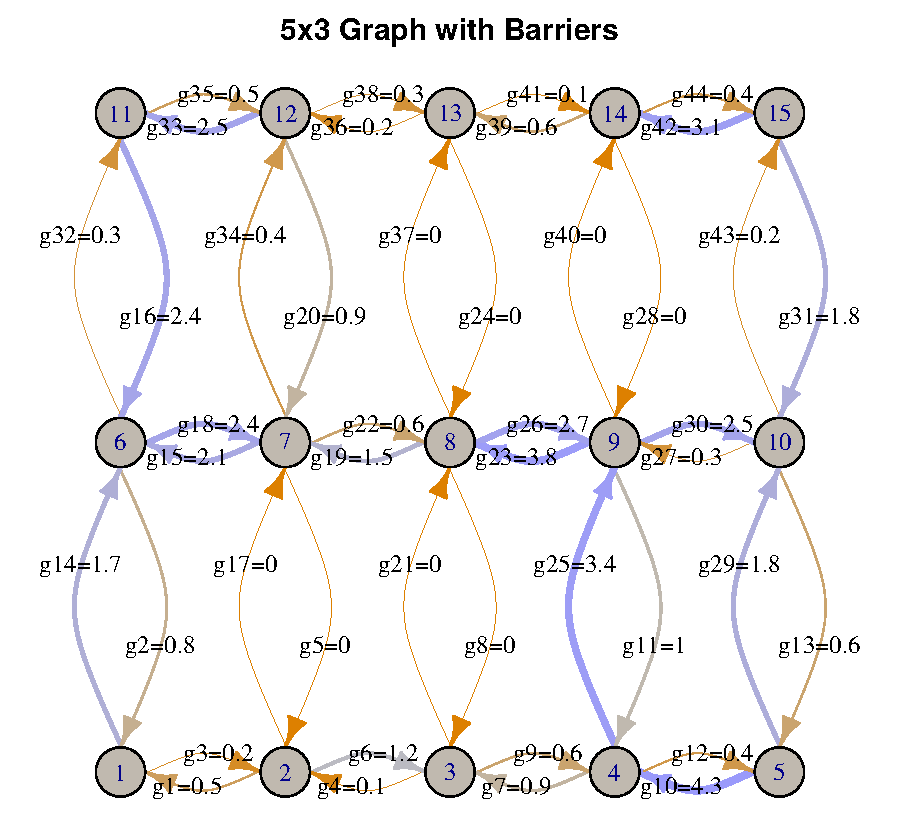
\includegraphics[width=0.6\textwidth]{figs/5x3b_grid}
    \caption{The grid structure and parameter labels
    for the 5 $\times$ 3 grid with two barriers:
    movement rates between $\{2,3\}$ and $\{7,8\}$ are zero,
    as are those between $\{8,9\}$ and $\{13,14\}$.
    Values for the non-zero movement rates 
    were chosen by rounding independent draws of an exponential random variable with mean 1 
    up to the nearest tenth.
    } \label{fig:5x3b_grid}
\end{figure}

\begin{figure}
\centering
     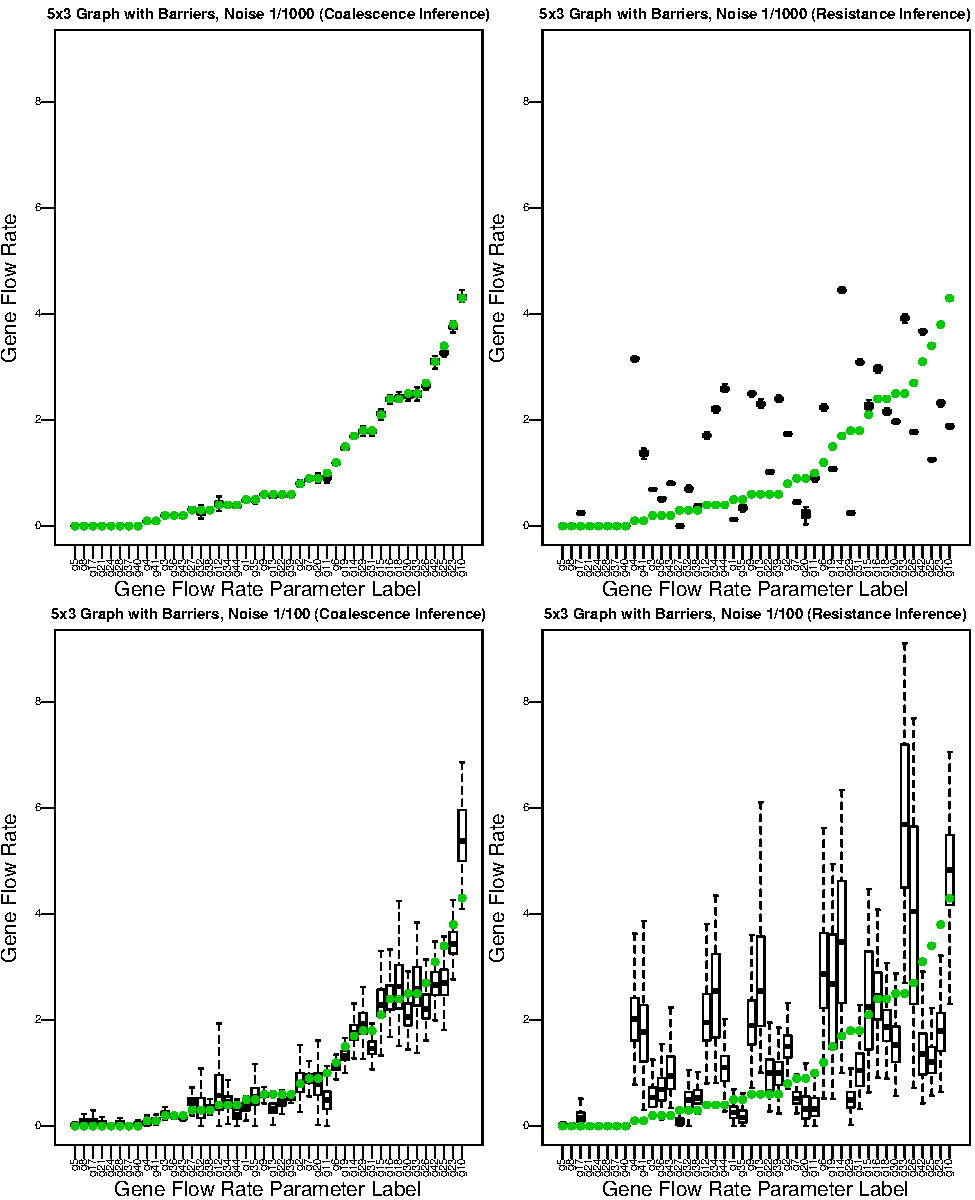
\includegraphics[scale=1]{figs/5x3b_post_coalvcom}
    \caption{
        Coalescence time inference is much more accurate than resistance inference:
        posterior distributions for gene flow rates in the 5 $\times$ 3 graph with barriers,
        compared to true values (in green),
        using \textbf{(left)} coalescence time and \textbf{(right)} resistance distance inference,
        with \textbf{(top)} low noise and \textbf{(bottom)} high noise,
        See Figure \ref{fig:5x3b_grid} to match parameter labels to positions on the graph.
    \label{fig:5x3b_post_coalvcom}
}
\end{figure}


%%%%%%%%%%%%%%%%%%%%%%%%%%%%%%
\subsection*{Biased migration}
\label{sec:biased_migration}

Both matrices of coalescence and commute times, $C$ and $R$, are symmetric,
but they do not deal with asymmetric (biased) migration in the same way.
Since commute time to location $i$ requires paths both to and from $i$,
but coalescence time to $i$ does not,
if there is a low rate of migration back into $i$,
then commute times to $i$ could be quite long even while coalescence times are not.
For instance, suppose there are three populations arranged in a line,
and lineages currently in the outer populations are much more likely to come from the central population
than the other way around.
Since lineages quickly move to the center and coalesce regardless of starting position, 
\llabel{ll:dense3}
coalescence time (and genetic diversity) will be relatively low between all individuals. \revpoint{4}{4}
Commute time between the two outer locations, on the other hand,
will be much longer than other comparisons, since it requires a lineage to leave the center.

In order to investigate this general situation,
we tested both methods on four different $4 \times 4$ graphs (shown in Figure \ref{fig:4x4_grids}):
\emph{uniform}, where all movement rates are 1.0;
\emph{symmetric}, where movement rates are symmetric ($G_{ij} = G_{ji}$)
and randomly generated as before;
\emph{asymmetric}, where all movement rates are random;
and \emph{biased}, where movement rates down or to the left are equal to 2.0,
and movement rates up or to the right are 0.5.
For inference, we added noise with standard deviation $1/500^\text{th}$ of the mean value.

Differences between true mean coalescence times ($C$) and mean resistance distances ($\comdist$)
are shown in Figure \ref{fig:RvsC}: \revpoint{1}{19}
they are fairly small in the uniform and symmetric cases, moderate in the asymmetric case, 
and extreme in the biased asymmetric case.
This difference suggests that resistance distance inference may be strongly misled \revpoint{2}{7}
in the asymmetric and biased situations,
but in principle it still could be the case that 
the movement rates that give the best fit of resistance distance
to coalescence time data could be close to the actual rates use to generate the data.
This does not seem to occur in practice:
coalescence time inference was substantially more accurate in all cases.
Posterior distributions of inferred movement parameters are shown in Figure \ref{fig:4x4box}.
The mean absolute errors for coalescence time inference are 0.12 or less in all cases.
Resistance distance inference obtains roughly uniform migration rates
(although varying by a factor of 2) in the uniform case;
and migration rates noisily correlated with the truth in the symmetric graph.
However, resistance distance inferences for the asymmetric and biased graphs are only weakly correlated, 
if at all, to the truth.
Resistance distance inference also drastically overestimates movement rates for the biased case,
as we would expect based on the differences discussed above.


\begin{figure}
\centering
     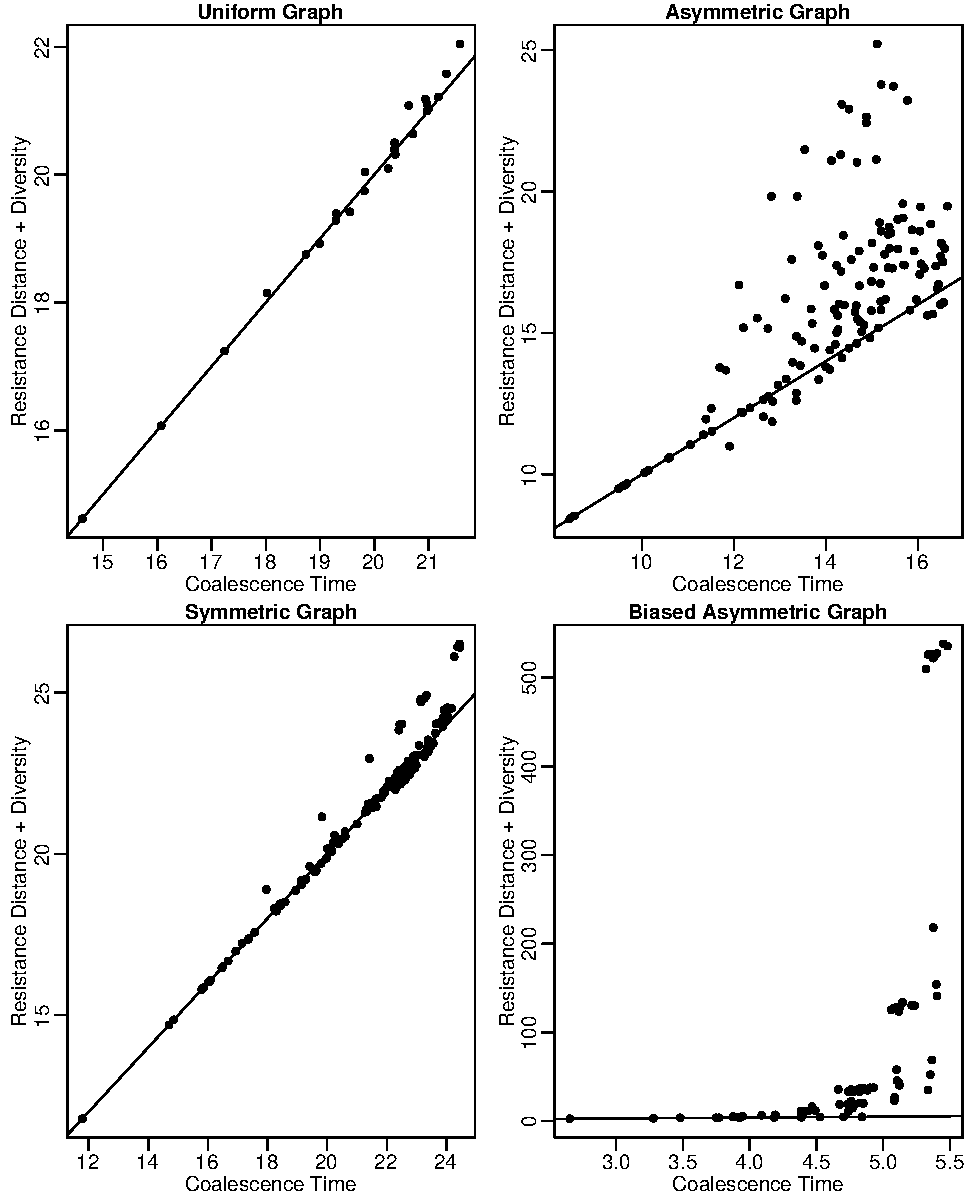
\includegraphics[scale=1]{figs/RvsC}
    \caption{
        Resistance distances ($\comdist$) compared to coalescence times ($C$)
        on the $4 \times 4$ graph, with 
        \textbf{(top left)} uniform movement rates,
        \textbf{(bottom left)} random, symmetric rates,
        \textbf{(top right)} random, asymmetric rates,
        and \textbf{(bottom right)} rates with a small diagonal bias (see text).
        The line shows $y=x$.
        See Figure \ref{fig:4x4_grids} for specific values and graph structure.
    \label{fig:RvsC}
}
\end{figure}

\begin{figure}
\centering
     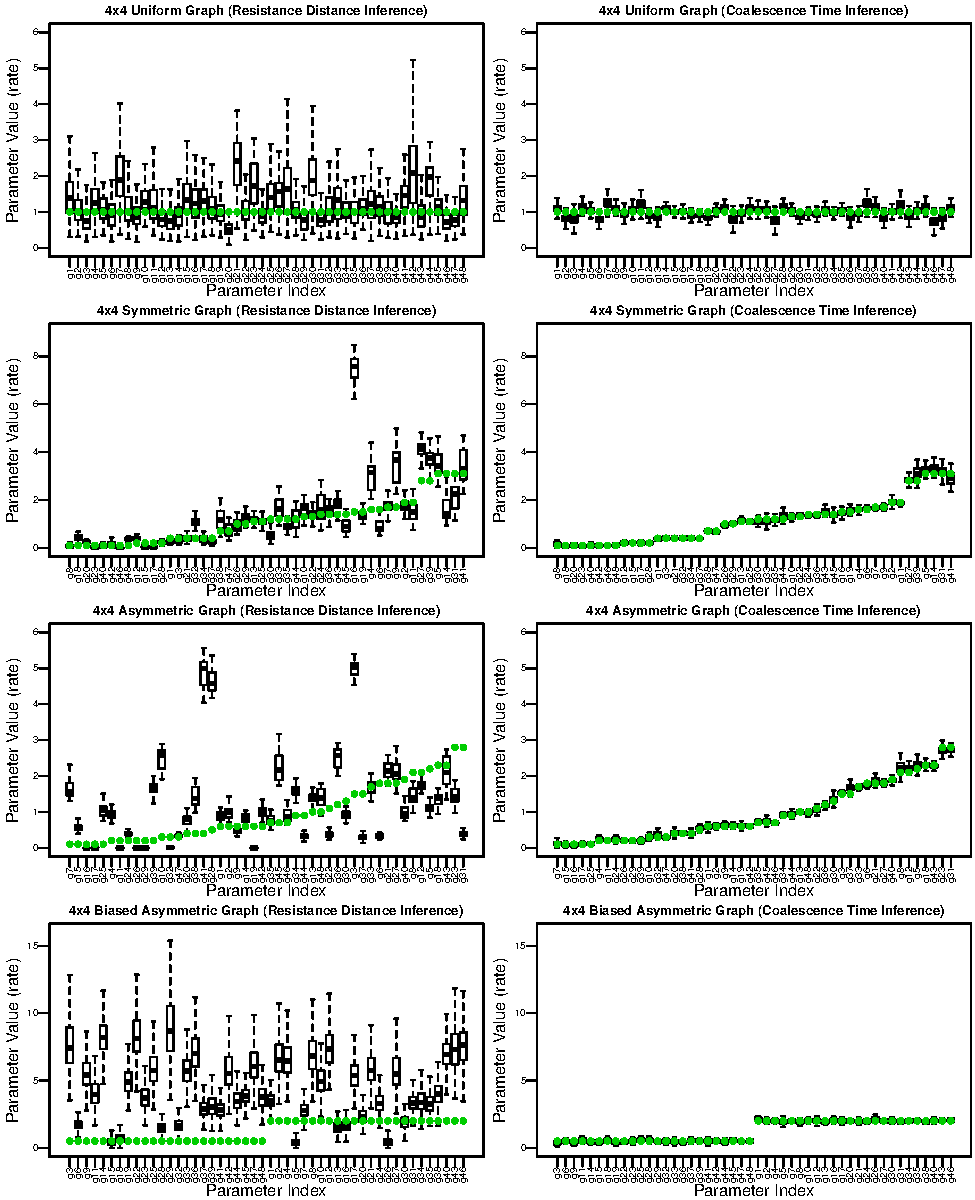
\includegraphics[scale=1]{figs/4x4coalvcom_paper}
    \caption{
        Boxplots of the posterior distributions of movement rates
        inferred using the
        \textbf{(left)} coalescence times
        and \textbf{(right)} resistance distances
        shown in Figure \ref{fig:RvsC};
        i.e., on the $4 \times 4$ graphs with
        \textbf{(top)} uniform,
        \textbf{(middle top)} symmetric,
        \textbf{(middle bottom)} asymmetric,
        and \textbf{(bottom)} biased
        movement rates.
        See Figure \ref{fig:4x4_grids} for specific values and graph structure.
    \label{fig:4x4box}
}
\end{figure}


%%%%%%%%%%%%%%%%%%%%%%%%%%%%%%%%%%%%%%%%%%%
\subsection*{Continuous geographical space}

The data we have used thus far are produced ``under the model'',
and should provide an accurate depiction of our method applied to discrete, randomly mating populations
whose connections by migration are known.
However, this is nearly always a rough approximation to reality,
in which organisms are distributed across continuous geography,
and ``populations'' are constructed by necessity, often driven by sampling locations.
For this reason, we applied coalescence and resistance inference,
as well as the resistance-based method EEMS \citep{petkova2016visualizing},
to data from simulations on continuous geography.

\paragraph{Process noise}
The mean coalescence times of lineages that we compute analytically
are exact for large, randomly mating populations,
but the word ``mean'' indicates an average across several levels of randomness:
each observed, empirical mean estimated using a sample of genotypes
will deviate from this depending on the individuals sampled (``individual sampling noise'')
\citep{ashander2018demographic},
the genetic loci genotyped (``genome sampling noise'') \citep{waples2009modelling},
and the stochasticity of the population history itself (``process noise'')
\citep{wakeley2012genealogies,waples2009modelling}.
% Both sources of noise can be substantially larger 
% in populations living across continuous geography
% than in discrete populations
% due to randomness in spatial locations.
% This is hinted at by Figure \ref{fig:5x3b_continuous},
% where we see that the distribution of individuals across the landscape is fairly patchy:
% a barrier might be inferred in a region that has not happened to have a local population recently
% only because of demographic stochasticity.
% This might make inference using a discretization of continuous space considerably more difficult.
Sequencing of many nonascertained loci genome-wide should minimize the second source of noise
(although genome structure can affect this at large scales \citep{li2016local}). \revpoint{3}{11}
Geographic models in continous space, 
are expected to show much more process noise than discrete population models
because of random fluctuations in local population density. \revpoint{3}{10}
To quantify the relative contributions of the remaining sources of noise,
we compared mean genetic distances, calculated in the same way,
between two nonoverlapping sets of samples from each of three identical simulations.
These forwards-time, continuous-space simulations were done using SLiM as described in the Methods.
We found that with these parameter values, process and sampling noise were of similar magnitude,
contributing 6.7\% and 13.8\% of the variance, respectively
(Supplemental Figure \ref{fig:h_val_comp}).
% An implication of this is that uncertainties in genetic distance
% estimated from the data will be (possibly large) underestimates,
% a fact also pointed out for effective population size by \citet{waples2009modelling}.


\paragraph{Biased migration}
% Although we found substantial process noise
% with a large, flat landscape with uniform, unbiased migration,
% many biological processes are expected to increase between-replicate stochasticity.
To test inference on a simple, continuous landscape with bias, 
we simulated a square, flat landscape as above,
but with \emph{biased migration}: 
each offspring's location was chosen randomly as before,
but with mean location $\sigma_d/10$
up and to the right of the parent's location.
% (or 0.05\% of the edge length of the landscape)
This again produces reverse-time gene flow down and to the left.
% As a population genetics model,
% this case is similar to a population expansion,
% replacing the leading edge of the expansion with the corner of landscape 
% that migration bias leads away from.
% In this situation, as in an expansion, 
% individuals at the edge may have disproportionately more offspring,
% leading to low genetic diversity and strong drift \citep{edmonds2004mutations,hallatschek2010life}.
% This results in substantially more noise in the data,
% clearly visible in the isolation by distance plots of Figure \ref{fig:ibd_comp}. 
% Despite this large contribution of process noise,
Coalescence time inference correctly infers the bias on a broad scale:
using a $4 \times 4$ grid,
inferred gene flow rates down and to the left are consistently much larger
than those up and to the right;
resistance distance-based results show no clear pattern
(Supplemental Figure \ref{fig:grid_bias_4x4_1}).
However, we do not obtain the clear picture of the landscape
we saw for the corresponding discrete-population model
(bottom-right plot, Figure \ref{fig:4x4box}):
inferred rates show substantial heterogeneity,
likely due to stochasticity of recent demography.


\paragraph{Identifying a barrier}
We now revisit the earlier situation where a landscape has locations that are barriers to gene flow.
The landscape is shown in Figure \ref{fig:5x3b_continuous},
where red bars depict uninhabitable regions that block migration.
Since the distribution of offspring locations is truncated at three standard deviations
away from the mother, a sufficiently thick uninhabitable area completely stops migration
directly across it.
We calculate mean genetic distances using 50 individuals 
from each grid location,
here giving us a total of 750 individuals.
The gene flow rates across the barriers are reliably estimated to be very small,
while other values have substantial variation:
in particular, gene flow rates are estimated to be low
across some edges that do not cross barriers;
this may be because of recent demographic stochasticity.
The barriers were also identified with comparable accuracy by both our resistance distance method
and EEMS, as shown in Supplemental Figure \ref{sfig:barrier_results}.
Note also that this analysis began by grouping samples into discrete ``populations'' appropriately;
in absence of a good \textit{a priori} idea of where barriers are,
this step might not be straightforward. \revpoint{2}{4}
To make parameters most easily interpretable,
geography should probably be discretized along natural barriers
and so that each region is of roughly the same geographic area.
% For instance, we may wonder whether a river or other geographical feature
% restricts gene flow.
% We would then discretize the landscape such that individuals on opposite sides of the 
% potential obstruction are in separate grid spaces.

\begin{figure}
\centering
     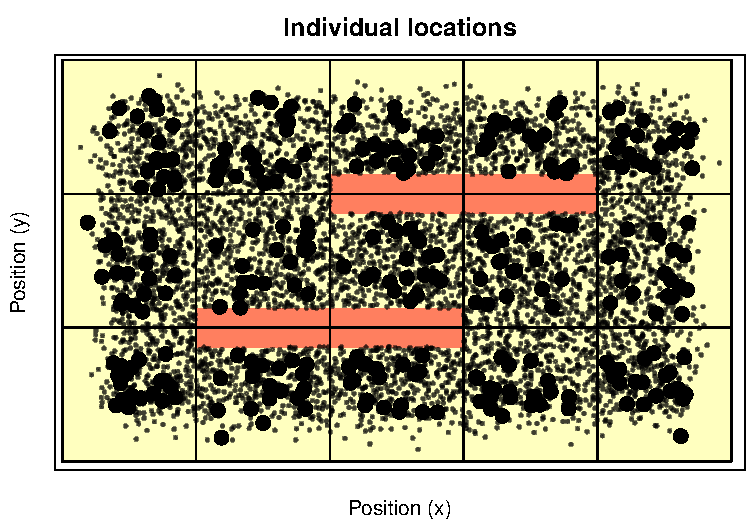
\includegraphics{{figs/barrier_sample_locations_pretty.fonts}.pdf}
     \includegraphics[height=0.3\textheight]{figs/barrier_coal_grid}
     \includegraphics[height=0.3\textheight]{figs/barrier_coal_boxplots}
    \caption{
        \textbf{(top)}
        Locations of individuals on the $5 \times 3$ landscape with barriers,
        with individuals used to compute the mean genetic distance matrix marked in bold.
        Red bars show uninhabitable regions,
        which are sufficiently thick so that no migration can occur directly across them.
        \textbf{(bottom left)}
        Posterior medians of movement rates inferred using coalescence time inference,
        and \textbf{(bottom right)}
        boxplots of corresponding posterior distributions,
        with movement rates crossing the barriers colored in red.
        The grouping of individuals into a $5 \times 3$ grid is shown above,
        and labels are the same as in Figure \ref{fig:5x3b_grid}.
    \label{fig:5x3b_continuous}
    }
\end{figure}


\paragraph{Other barriers: population sinks and recent expansions}
We simulated two other situations on a continuous landscape that produced an bias in effective migration.
First, we simulated a \textbf{valley} in a landscape with a $5 \times 3$ aspect ratio as above, 
in which fecundity of individuals in the middle 1/4 of the landscape was reduced by 50\%.
The valley is a population ``sink'',
although it would not be detectable with mortality rates,
and shows only a slightly lower population density (Supplemental Figure \ref{sfig:valley_results}).
Since individuals in the valley are more likely to have parents outside of the valley,
this produces gene flow ``uphill'', away from the ridge.
Next, we simulated a recent \textbf{expansion},
in which the middle 4/5 of the landscape was uninhabitable for 400,000 generations, \revpoint{1}{18}
until 500 generations before the present day.
(This is a model of secondary contact with a long period of isolation,
but not outside the realm of possibility.)
The resulting expansion produces gene flow back away from the center,
similar to the ``valley''.

Both coalescence time inference and the resistance landscape inferred by EEMS
show a barrier to gene flow in the middle of the landscape (Figure \ref{fig:more_barriers}).
This is arguably correct, 
although there is in fact no current barrier to migration in either simulation.
Coalescence time inference also correctly infers 
the general bias in recent gene flow away from the center,
although as in other continuous-space simulations, 
there was substantial noise in the inferred patterns.
However, the resistance landscapes as inferred by EEMS show patchy, vertical bands of high resistance.
These patterns are commonly seen when attempting to use EEMS, 
whose underlying model of gene flow is symmetric,
to describe anisotropic gene flow.
The grid-like pattern visible in this and other EEMS results
may be due to the sampling scheme
(recall that samples are drawn from the middle three-quarters of each grid square). \revpoint{1}{20}
Our analysis above shows that this is an unavoidable consequence of the resistance approximation,
and our implementation of resistance distance inference,
which allows asymmetric gene flow, shows similar patterns
(Supplemental Figures \ref{sfig:valley_results} and \ref{sfig:expansion_results}).

\begin{figure}
\centering
    \includegraphics[width=0.45\textwidth]{figs/valley_eems}
    \includegraphics[width=0.45\textwidth]{figs/valley_coal_graph}
    \includegraphics[width=0.45\textwidth]{figs/expansion_eems}
    \includegraphics[width=0.45\textwidth]{figs/expansion_coal_graph}
    \caption{
        \textbf{(Left:)}
        resistance landscapes inferred by EEMS
        and 
        \textbf{(right:)}
        gene flow rates inferred using coalescence time inference,
        from individual-based simulations on a continuous landscape,
        with \textbf{(top)} a \emph{valley} of reduced fecundity in the middle, and
        \textbf{(bottom)} a recent \emph{population expansion} from both edges of the range
        that met in the middle.
        The color scale shows the posterior mean log migration rates inferred by EEMS.
        \label{fig:more_barriers}
    }
\end{figure}

%%%%%%%%%%%%%
\subsection*{Application to \textit{Populus}}

Our discretization of the sampling area for the two poplar species
is shown in Figure~\ref{fig:poplar_results},
along with arrows depicting posterior mean estimates of gene flow.
Posterior distributions of gene flow rates and coalescence rates
are shown in Supplemental Figures~\ref{sfig:poplar_g} and \ref{sfig:poplar_gam}.
The main features of the resulting model are:
(a) low but nonzero gene flow between species,
with the highest rate between regions 3 and 4;
(b) strong bias in gene flow among (inland) \textit{balsamifera} regions,
from southeast to northwest ($3 \to 5 \to 6 \to 1$); and 
(c) strong bias in gene flow into regions 2 and 8.
These results align with what is known about \textit{Populus} history and ecology in the region
(personal communication, A.~Moreno Geraldes and Q.~Cronk, and \citet{geraldes2014landscape}).
There is ongoing hybridization around region 4,
and interspecific gene flow from 9 to 3 may be due to downstream transport along the Columbia river
(A larger gene flow rate from 9 to 3 indicates that individuals in region 9
are more likely to have recent ancestry in region 3 than vice-versa.)
The glacial refugia for the two species are thought to be in western Alaska (\textit{balsamifera})
and coastal British Columbia (\textit{trichocarpa}).
Inferred gene flow leading back towards these regions (depicted by larger arrows on the map)
are consistent with this --
for instance, if region 5 was colonized from region 6 sufficiently recently,
then individuals in region 5 should trace their ancestry to region 6 much more frequently
than vice-versa, as indicated by the large $5 \to 6$ arrow 
and small $6 \to 5$ arrow in Figure~\ref{fig:poplar_results}.

Interpreting these results requires some nuance beyond what was necessary in our simulation results.
Sampling locations are sparse, especially in the inland species,
so how exactly should we think of the geographic extent of ``region 6'',
which is represented by only two, distant samples?
Is this region's low inferred coalescence rate
a result of simply a large population (due to a large geographic region)
or barriers to movement within the region?
Although it is not entirely clear how to translate discrete-population models
to continuous space, \llabel{ll:continuous}
a ``gene flow rate'' from region $i$ to region $j$ as shown in Figure~\ref{fig:poplar_results}
is best thought of as an estimate of the proportion of the individuals in region $i$
that have a parent in region $j$, averaged over time and scaled by some unknown factor.
Equivalently,
this is the probability per unit time
that a lineage traced back from an individual in region $i$ follows a line of descent to region $j$,
again scaled by some factor.
We therefore expect gene flow to be biased from an area of 
lower population density (or, net fecundity)
into a neighboring region of higher population density.
We also expect gene flow to be biased 
from a smaller region to a larger, neighboring one than vice-versa
if a larger proprotion of the smaller region lies close to the boundary between the two.
This may explain the net bias from many coastal populations to inland ones.
We grouped samples so that each group represented roughly comparable geographic regions,
to ameliorate these confounding factors. \llabel{ll:discretization}
However, these difficulties in interpretation are common in any situation
where discrete populations are used to model continuous geography.

\begin{figure}
\centering
    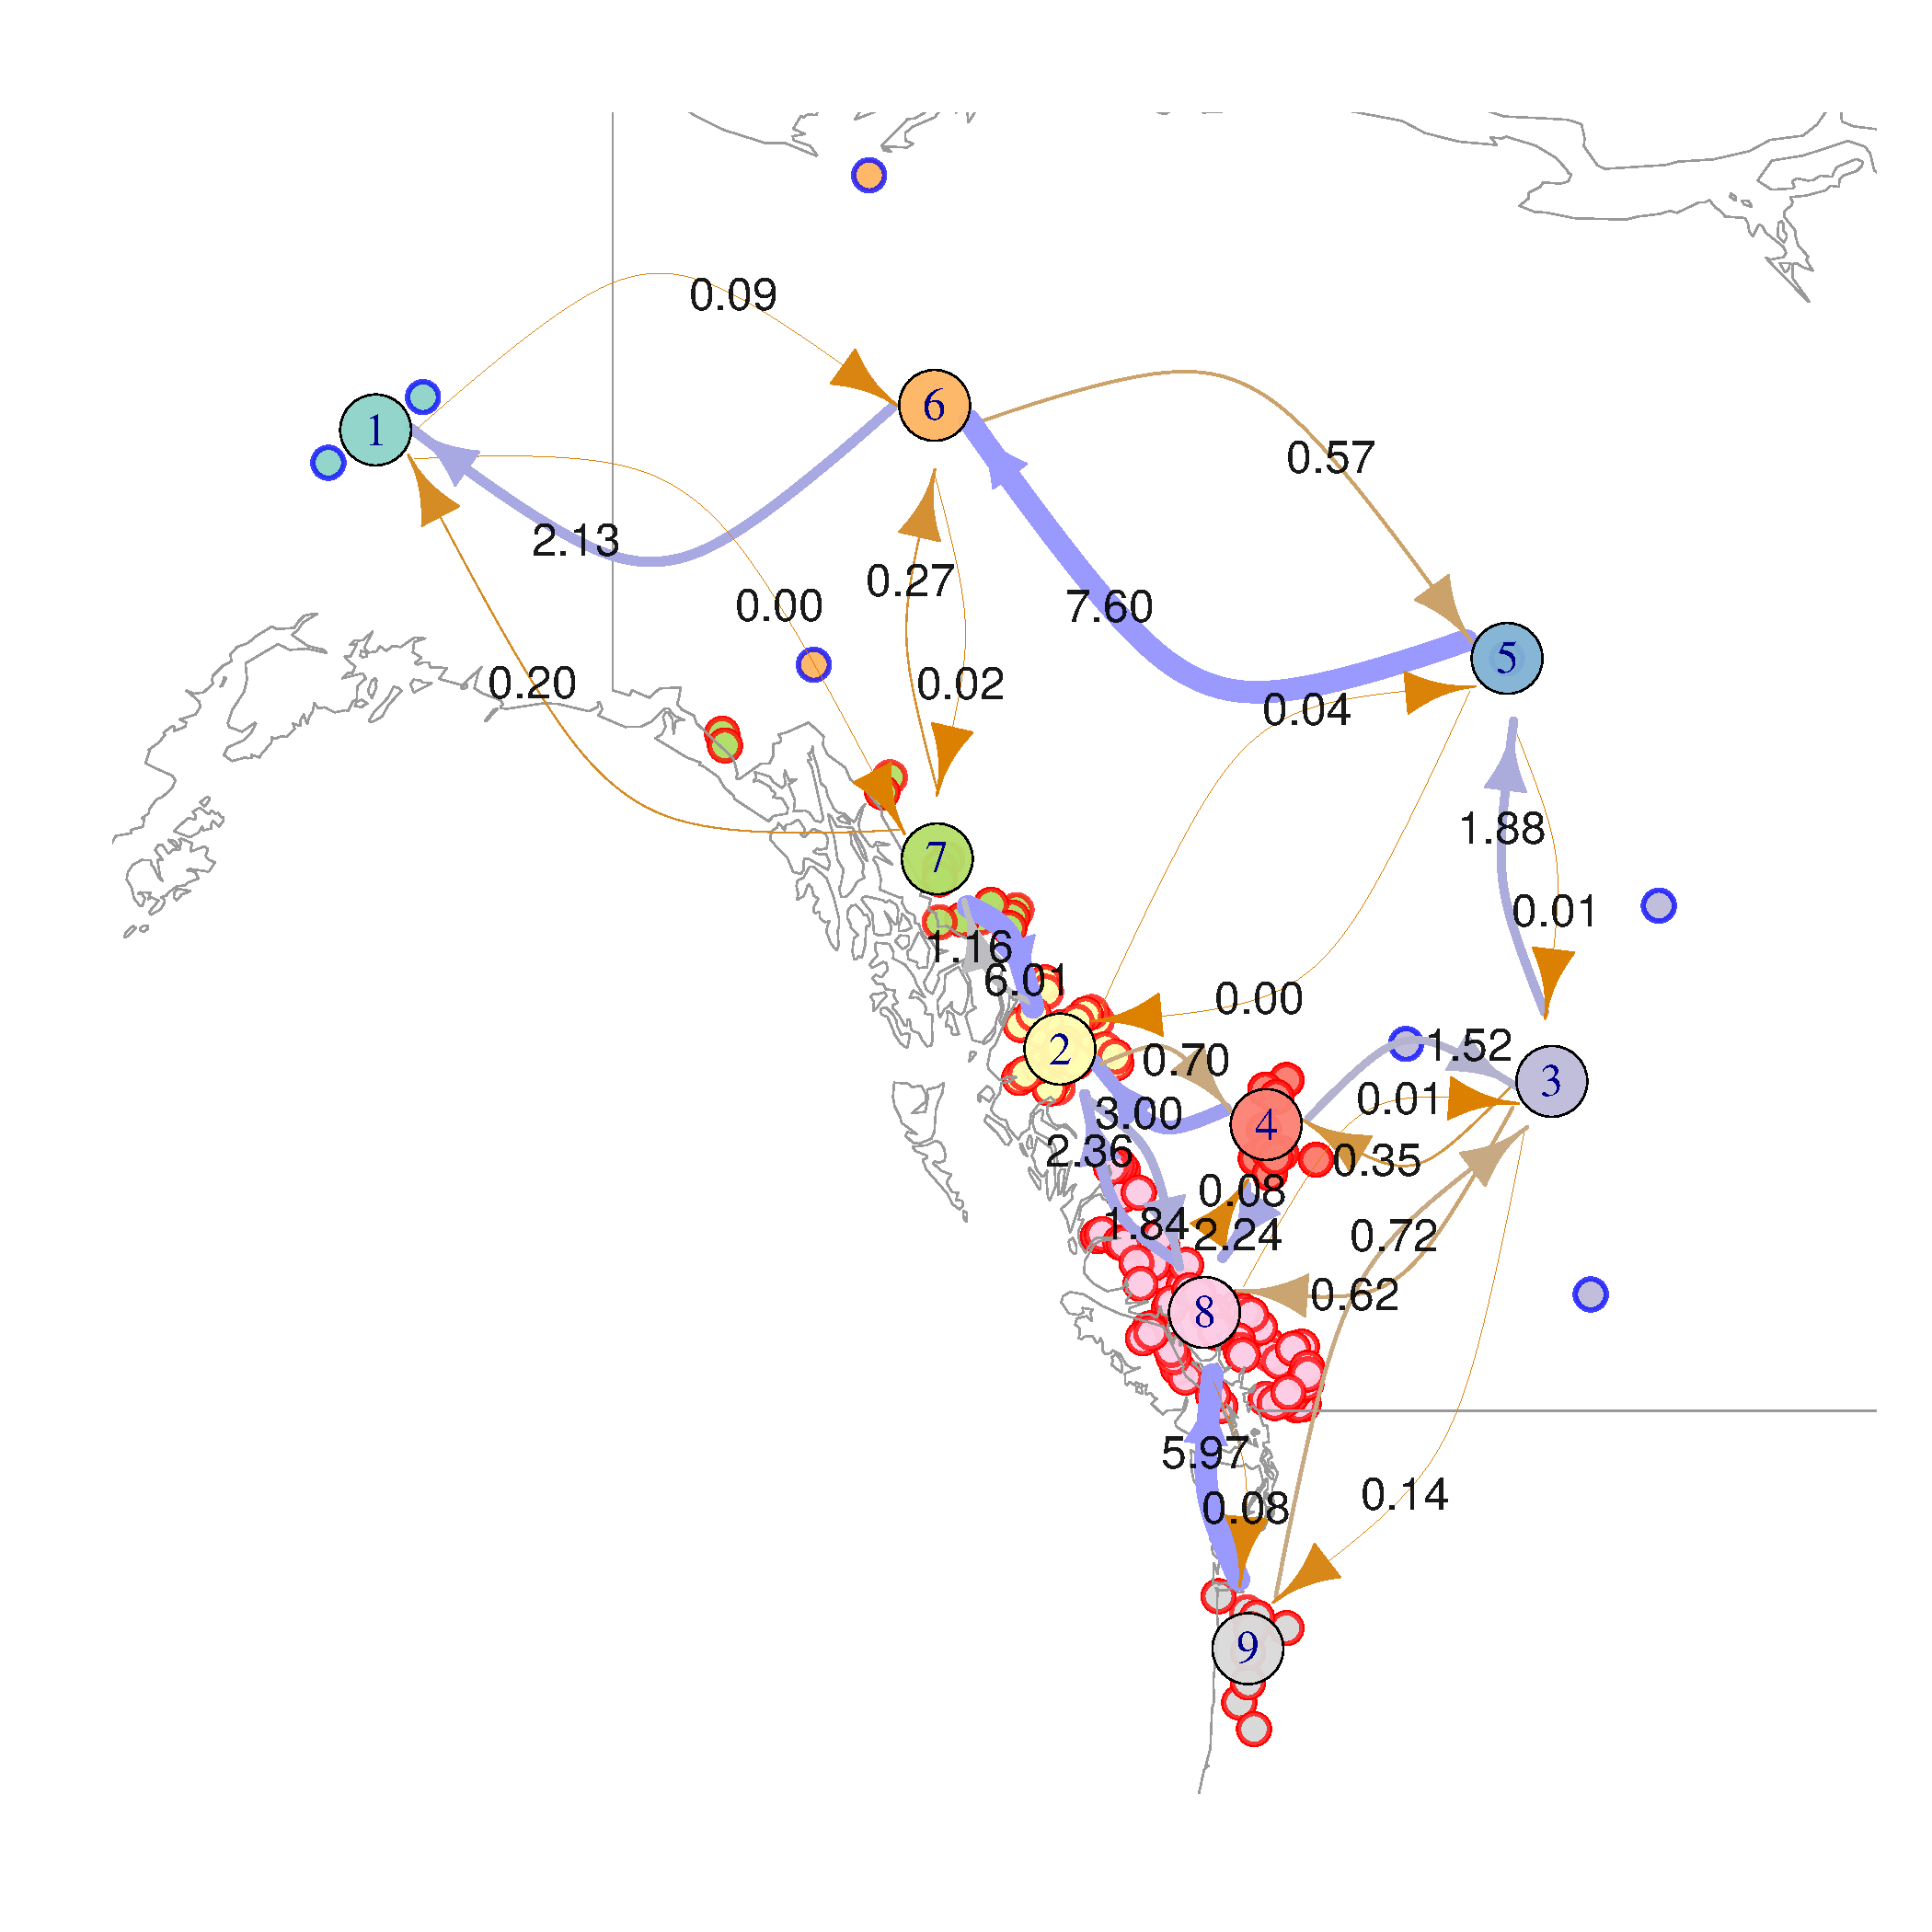
\includegraphics[width=0.9\textwidth]{poplars/grid_populus_map}
    \caption{
        Model results for \textit{Populus} data,
        superimposed on a map of northwestern North America.
        Sampling locations of \textit{Populus} genomes are small circles,
        with outer color indicating species 
        (red-outlined, coastal samples are \textit{trichocarpa}, 
        blue-outlined, inland samples are \textit{balsamifera});
        circle fill color indicates how samples are grouped into discrete ``populations''.
        Large circles are placed at group centroids, and given group labels.
        Arrow width is proportional to the posterior mean gene flow rate inferred under
        the coalescence time model (also given by the labels):
        for instance, the inferred gene flow rate from 4 to 2 is 3.0,
        while that from 2 to 4 is 0.7,
        suggesting that poplars in region 4
        have many more recent ancestors in region 2
        than poplars in region 2 do in region 4.
        Northwestern bias in gene flow between \textit{balsamifera} regions
        may reflect postglacial expansion to the south and east out of a refugium in Alaska.
        \label{fig:poplar_results}
    }
\end{figure}

%%%%%%%%%%%%%%%%%%%%
\section*{Discussion}

In this paper, we study how to 
use genetic and geographic distances between present-day samples
to infer the demographic parameters of a population that lives across
a heterogeneous two-dimensional landscape.
In particular, we have shown that the resistance distance approximation
-- which underlies several of the most commonly-used tools of landscape genetics --
can produce erroneous estimates, especially in the presence of biased gene flow.
We implement an alternative method, 
which uses coalescence times instead of the resistance distance approximation,
which provides good estimates of gene flow in a wider range of situations
(Figures \ref{fig:5x3b_post_coalvcom} and \ref{fig:4x4box}).
This weakness of resistance-based methods is not surprising --
the original papers 
describing Circuitscape \citep{mcrae2006isolation} and EEMS \citep{petkova2016visualizing}
present the resistance approximation as a necessary step for computational feasibility. \llabel{ll:approx}
Results of resistance-based methods should therefore be interpreted with caution:
for example, high inferred gene flow between two areas
may actually mean the areas are being fed by a common source.

Our new method infers effective population sizes and gene flow rates quite well 
-- and, being Bayesian, provides estimates of uncertainty --
given data from discrete populations connected by migration.
Can our method replace resistance-based methods? 
Perhaps, but
the substantial uncertainty we saw on graphs with only tens of nodes
is indicative of a larger problem we face for realistic models.
We have seen that discretization of space results in substantial modeling error,
in part because of randomness of geographic sampling
and unmodeled process noise can lead to overfitting.
Partitioning space into a finer grid should help with these problems,
but tends to make the inference problem itself more ill-conditioned:
with more connections,
changing the value of one connection affects coalescence time less,
and so inferences about that value must necessarily be less certain.
This tradeoff implies some degree of unavoidable uncertainty.
Reproducible, reliable inference will likely require development of new inference methods
that explicitly model continuous geography.
In the meantime, comparison of results utilizing different discretizations of geography
can help identify problems.  \revpoint{3}{12}


Although commute and coalescence times can be quite different,
they are equal (with a particular choice of local diversity)
if populations are arranged on a ring or torus
with symmetric migration
(as also noted by \citet{mcrae2006isolation}).
The similarity of these models to rectangular grids
may explain why in other work, resistance distance methods have shown relatively good fit to data
simulated with symmetric migration rates.


\paragraph{Other methods}
For comparison on equal footing, we have implemented a resistance-based inference method.
However, methods that use resistance distance have substantial advantages over the method we present here.
Circuitscape \citep{mcrae2008using} produces maps of much higher resolution 
than is presently possible with coalescent times. \revpoint{4}{1}
\citet{hanks2013circuit} connects the problem to intrinsic conditional autoregressive models, 
providing a Bayesian model of an underlying Gaussian Markov random field.
EEMS \citep{petkova2014visualizing} integrates over possible tessellations of the region
as a way of regularizing the inferred landscape,
aiming to obtain a map at the best possible resolution supported by the data.

Most promisingly, the recent method, MAPS \citep[``Migration and Population Surface estimation'',][]{alasadi2018estimating}
is based on EEMS, but instead of resistance distances,
uses pairwise sharing of long haplotype segments,
which have been shown to carry substantial information about recent demography
\citep{ralph2013geography,palamara2013inference,browning2015accurate,ringbauer2017inferring}.
Furthermore, the likelihood model underlying MAPS is based on coalescent theory,
and thus should not be subject to the drawbacks of resistance distance.
\citet{ringbauer2018estimating} also uses shared haplotype lengths
to identify a barrier in a coalescence-based framework.
However, the underlying migration model is symmetric,
and haplotype length-based methods require fairly dense genotyping and a genetic map,
something not available for many species.

Other widely-used inference methods, such as
MIGRATE \citep{beerli1999maximumlikelihood,beerli2010unified},
BayesAss \citep{wilson2003bayesian}, 
and IMa \citep{hey2007integration}
use likelihoods for the joint frequency spectrum derived from a coalescent model --
and so in principle could use much more of the data than our method,
which only uses pairwise divergences.
However, because they use locus-specific data rather than an average across loci,
these methods can only be applied to a relatively small number of populations and loci,
because of computational efficiency.
We have found asymmetry in migration rates to be important:
\citet{hanks2017modeling} developed a method that allows asymmetry
by modeling genetic similarity as deriving from an underlying random field
whose space-time covariance is given by the covariance of the (forwards-time) population fluctuations.
However, this is not motivated by a generative model for genetic data.

All of the methods presented above work with a discretized model of space,
for mathematical and computational reasons. \revpoint{5}{8}
Development of new methods for continuous geography
and assessment of how current methods behave when faced with continuous geography
is an important challenge facing the field.
This has been made substantially easier with the introduction of continuous space 
into the simulator, SLiM \citep{haller2018forward},
that we used to test the behavior of our method with more realistic data.
Another promising approach centers around the Spatial Lambda-Fleming-Viot model
\citep{barton2010continuum}, \revpoint{5}{9}
which provides a mechanistic model in which coalescent simulations are possible.
This has been used for inference \citep{guindon2016demographic},
but more work remains to understand how it behaves as an approximation to real populations.


\paragraph{Asymmetric dispersal and consequences for resistance methods}
We have found that asymmetric rates of lineage movement
can produce qualitative differences between coalescence times and resistance distances,
and thereby mislead models based on resistance distance.
How should this affect the results of resistance-based methods to genomic data,
besides general inaccuracy?
This asymmetry occurs if one region receives a greater proportion of each new generation as migrants
from another population than that other population does from it.
This is expected, for instance,
if organismal dispersal is biased by wind or water currents \citep{gaines2003avoiding,morrissey2009maintenance},
or in the presence of source-sink dynamics \citep{dias1996sources,lenormand2002limits}.
Suppose, for instance, that seed dispersal for a species of tree
is biased downhill,
and the landscape is dominated by a large valley.
Since lineages tend to move uphill,
genetic distance between locations on opposite slopes of the valley will be relatively large,
so resistance methods will infer a barrier along the bottom of the valley
when no barrier to dispersal exists.
On the other hand, if there is a ridge instead of a valley,
resistance methods will show no barrier (and relatively high movement rates),
even if there is very little uphill dispersal.
This could lead to a falsely high assessment of gene flow across the top of the ridge.

\paragraph{Circuitscape} \llabel{ll:circuitscape}
Could we use coalescence time in place of commute time
for workflows that compute values on a given map of movement rates
that are then compared to genetic distance?
In principle this could be done,
but there is no clear way to do this 
at the same (impressively fine) geographic resolution that is currently possible,
e.g., using Circuitscape \citep{mcrae2006isolation}.
This is because if we have $n$ sampled locations
on a landscape discretized into $N$ regions,
the computational complexity of finding commute times is $nN$,
but coalescence time scales as $N^2$
(Each $N$-vector of hitting times to a particular location can be found independently,
but the entire $N \times N$ matrix of coalescence times must be found together.)
However, as we discuss above, this fine geographic resolution is in some sense illusory --
for each fine-resolution map there should be coarser maps that give almost identical coalescence times --
but we are not aware of existing theory providing guidance on how to find these.

\paragraph{Difficulty of inference}
What determines the feasibility of inferring movement rates from genetic distances?
Using coalescence times instead of commute times greatly improves accuracy in many situations,
but there are still a number of factors that determine the tractability of the problem.
Observation noise is clearly an issue:
we found that estimation errors of a few percent was enough to seriously degrade accuracy.
However, genetic distances can be estimated to much higher accuracy using modern genomic data.
Perhaps more seriously,
a low rate of coalescence relative to movement can also make the problem essentially nonidentifiable.
This is clear at least in the limit: with very low coalescence, 
the population loses any isolation by distance and is indistinguishable from a randomly mating population.
In continuous landscapes, this balance is measured by Wright's local effective population size,
which is proportional to the number of other individuals 
within a circle of radius equal to the mean dispersal distance.

Inference of movement rates, in either a coalescence time or resistance distance framework,
is an ill-conditioned problem,
implying the need for regularization to obtain reliable inference.
This fact could explain the results of \citet{graves2013current},
who found a large area of resistance parameters
that produced equivalently good fits to genetic distance
(i.e., nonidentifiability, analogous to a flat likelihood surface).
An anonymous reviewer suggested
that although inference of landscapes of movement rates may carry a degree of unavoidable uncertainty,
the problem of \emph{model comparison} 
(e.g., between models with and without migration across a certain barrier)
may still produce more certain answers. \revpoint{2}{2}

Computation time currently limits this method to a discretization of less than 30 populations,
but nonidentifiability is probably a more serious barrier that must be concurrently addressed
before scaling the method to finer discretizations of space. \llabel{ll:computation}
Finer discretizations of space should benefit from the use of sparse matrix methods,
but in our testing these did not speed up computation at this scale. \revpoint{1}{2}

\paragraph{The effect of history} \llabel{ll:history}
The models we discuss here assume that population sizes and migration rates
have been constant on the time scale given by the within-species coalescent time.
This is rarely true in practice \citep{neigel1991estimation,barton1995genealogies}.
However, geographic differences in mean relatedness
are established on a shorter time scale --
the time scale over which a lineage, moving randomly across the landscape,
``forgets'' where it started
(i.e., the mixing time of the Markov chain \citep{wilkins2004separationoftimescales}).
This is the time it takes for the uncertainty in lineage movement
to reach the scale of the species range.
For instance,
if the width of a species' range is roughly 500km,
and if mean dispersal distance is 10km,
the standard deviation of ancestor location $t$ generations ago is $10\sqrt{t}$,
so the mixing time of a lineages across the landscape,
not accounting for barriers, is of order 2500 generations.
The habitat of many species would have changed substantially over this time, % \citep{pleistocene_mojave}
which suggests that models incorporating change over time 
may be required to model modern diversity.
However, the effects of recent history are strongest,
so landscapes estimated assuming constant populations
may give a reasonable picture of the landscape averaged over recent times.


\paragraph{Assumptions}
Modeling lineages as a Markov chain is nearly ubiquitous in population genetics today,
but may not be appropriate.
Even if the population dynamics in forwards time are Markov, 
the dynamics of lineages traced back in time (the coalescent process) may not be. 
For example, if individual fecundity is variable and population density is low,  \revpoint{3}{15}
two lineages near each other are more likely to share a recent common origin, 
so knowing how one lineage moves is informative about how the other lineage is likely to move. 
This effect becomes small as population density increases, 
so it should be a relatively minor point if the offspring
of any one parent are typically interspersed with the offspring of many others. 
Natural selection also makes the coalescent process non-Markovian.
Differences in the strength of linked selection along the genome
could even cause the statistical behavior of lineages to depend
on the region of the genome being studied \citep{wang2014isolation,li2016local}.
However, more investigation with continuous-space models is needed.



%%%%%%%%%%%%%%%%%%%%%%%%%%%
\section*{Acknowledgements}

Thanks to David Levin for useful suggestions regarding hitting time calculations,
to Paul Marjoram for useful comments,
to Brad Shaffer and Evan McCartney-Melstad for discussions about landscape modeling,
to John Novembre, Hussein Al-Asadi and Benjamin Peter for help with EEMS
and general input,
and to Quentin Cronk and Armando Moreno Geraldes for consultations about the \emph{Populus} results.
We would also like to gratefully acknowledge the immense positive impact that Brad McRae \citep[1966--2017;][]{lawler2018tribute}
has had on landscape genetics and conservation biology through the introduction of landscape resistance.
We hope this paper helps to carry forward this work.
Work on this project was supported by funding from
the Sloan Foundation and the NSF (under DBI-1262645) to PR.


\bibliography{references}

\ifsubmission
\processdelayedfloats
\fi

\newpage


\appendix
\renewcommand{\thefigure}{S\arabic{figure}}
\setcounter{figure}{0}
\ifsubmission
    % for endfloat
    \renewcommand{\thepostfigure}{S\arabic{postfigure}}
    \setcounter{postfigure}{0}
\fi


%%%%%%%%%%%%%%%%%%%%%%%%%%%%%%%%%%
\section{The simplest example}
\label{ss:simple_example}

To demonstrate the main theoretical ideas,
we provide a short example.
Consider a Markov chain with two states, 
where the rate of movement from state 1 to state 2 is $G_{12}$
and the rate of movement from state 2 to state 1 is $G_{21}$,
so the generator matrix is
\begin{align*}
G = 
    \begin{bmatrix}
        -G_{12}  & G_{12} \\
         G_{21}  & -G_{21}
    \end{bmatrix}.
\end{align*}
Equation \ref{eqn:C_matrix} equates two $2 \times 2$ matrices,
so provides four equations. Only three of these are unique;
simplifying these and using that $C_{12} = C_{21}$, these are:
\begin{align*}
    2 \left(C_{12} - C_{11} \right) G_{12} - C_{11} \gamma_1 &= -1 \\
    \left(C_{11} - C_{12} \right) G_{21} + \left(C_{22} - C_{12}\right) G_{12} &= -1 \\
    2 \left( C_{12} - C_{22} \right) G_{21} - C_{22} \gamma_2 &= -1 .
\end{align*}
Given $C$, we have three equations for the four unknowns, 
$G_{12}$, $G_{21}$, $\gamma_{1}$, and $\gamma_{2}$,
which we can solve symbolically.
The valid solutions to these equations are those with $G_{12}$, $G_{21}$, $\gamma_1$,
and $\gamma_2$ nonnegative.
If $C_{11} \neq C_{12}$, 
we can write the solution with $\gamma_1$ as the free variable:
\begin{align*}
G_{12} &= \frac{1}{2(C_{11} - C_{12})} - \frac{C_{11}}{2(C_{11} - C_{12})}\gamma_1 \\
G_{21} &= \frac{-2(C_{11} - C_{12}) + (C_{12} - C_{22})}{2(C_{11} - C_{12})^2}
	- \frac{C_{11}(C_{12} - C_{22})}{2(C_{11} - C_{12})^2}\gamma_1 \\
\gamma_2 &= \frac{(C_{11} - 2C_{12} + C_{22})^2}{C_{22}(C_{11} - C_{12})^2}
	- \frac{C_{11}(C_{12} - C_{22})^2}{C_{22}(C_{11} - C_{12})^2}\gamma_1.
\end{align*}
This implies that $\gamma_2$ decreases as $\gamma_1$ increases as long as $C_{12} \neq C_{22}$.
This makes sense because
increasing a rate of coalescence cannot make expected coalescence times longer,
so in order to keep coalescence times the same,
if one coalescence rate is increased, another must be decreased.
This also implies that, in order for $\gamma_2$ to be a value other than $0$, 
we must have $C_{11} - 2C_{12} + C_{22} \neq 0$.
In general, if there is a value or range of values of $\gamma_1$
for which the other movement and coalescence parameters are non-negative,
then a solution exists.

\begin{figure}
\centering
         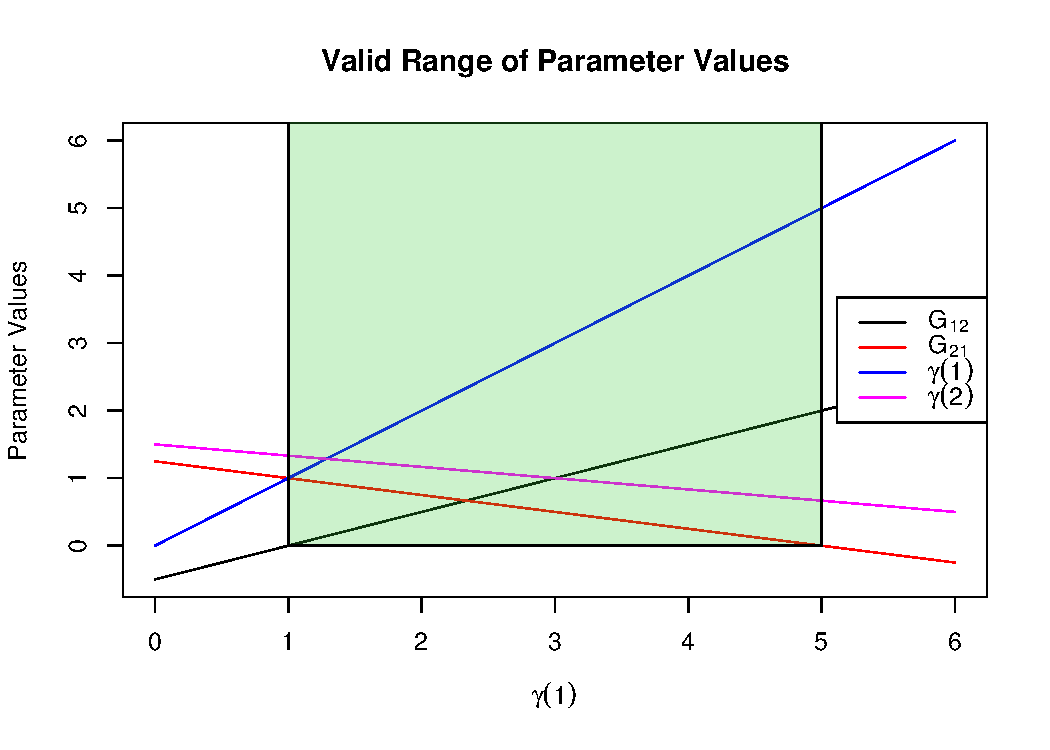
\includegraphics[scale=.7]{figs/valid_range}
    \caption{The green shaded region shows 
        the valid range of the parameter values
        for the two state Markov chain given that
        $C_{11}=1$, $C_{12}=2$, and $C_{22}=1.5$}
    \label{fig:valid_range}
\end{figure}

To produce a concrete example, suppose that
$C_{11} = 1$, $C_{12} = 2$, and $C_{22} = 1.5$ in arbitrary time units.
The other parameters will be non-negative 
when $1 \leq \gamma_1 \leq 5$,
as shown in in Figure \ref{fig:valid_range}.
Assuming $\gamma_1 = \gamma_2$ produces a unique solution, 
with $\gamma_1 = \gamma_2 = 1.29$ and $G_{12} = 0.14$ and $G_{21} = 0.93$.



%%%%%%%%%%%%%%%%%%%%%%%%%%%%%%
\section{Finding $G$ from $H$}
\label{apx::hitting_calcs}

Suppose that $G$ is the generator matrix of an irreducible continuous-time Markov chain $X$
on at least two states,
so that $G_{ij} \ge 0$ for $i \neq j$ and $G \bone = 0$.
Under these assumptions, there is a unique stationary distribution, $\pi$,
that satisfies $\pi^T \bone = 1$ and $\pi^T G = 0$.
Let $\tau_{j} = \inf\{t \ge 0 : X_t = j\}$ and $H_{ij} = \E[\tau_j \,|\, X_0 = i]$.
Then we know that
\begin{align*}
    (G H)_{ij} = -1 \qquad \text{for} \; i \neq j ,
\end{align*}
and hence that for some vector $x$,
\begin{align} \label{eqn:GH}
    GH = - \bone \bone^T + \diag(x).
\end{align}
What is $x$?  
First note that the Random Target Lemma \citep{aldous-fill-2014}
% https://www.stat.berkeley.edu/users/aldous/RWG/Book_Ralph/Ch2.S2.html
tells us that if $\pi$ is the stationary distribution of the chain, then 
$(H \pi)_i$ does not depend on $i$,
and so there exists a vector $\nu \propto \pi$
such that $H \nu = \bone$.
Multiplying equation \eqref{eqn:GH} by $\nu$, we get that
\begin{align*}
    0 = G\bone 
    = (\diag(x) - \bone \bone^T) \nu ,
\end{align*}
which rearranges to
\begin{align*}
    x_i = \frac{ \bone^T \nu }{ \nu_i } .
\end{align*}
But, since $\nu \propto \pi$,
it must be that $\pi = \nu / \bone^T \nu$,
and so $x_i = 1/\pi_i$.

Now, we prove that $H$ is in fact invertible, \llabel{rr:H_invertible}
by showing that $z^T H \neq 0$ for every nonzero vector $z$.
First note that $\bone^T H \neq 0$, since the entries of $H$ are nonnegative.
Now take $z$ orthogonal to $\bone$.
Since the chain is irreducible,
the eigenspace associated with the eigenvalue 0 for $G$ has multiplicity one,
and so any vector $y$ that satisfies $y^T G = 0$ is proportional to $\pi$.
This implies that there is a vector $y$ such that $y^T G = z^T$.
Multiplying equation \eqref{eqn:GH} on the left by $y^T$ obtains
$z^T H = y^T (\diag(1/\pi) - \bone \bone^T)$.
If $H$ is not invertible, then there is a $z$ for which this is zero,
i.e., $y_i / \pi_i = \sum_j y_j$ for every $i$.
But, this only holds if $y = \pi$, which was disallowed,
because then we would have $z = 0$.
Therefore, $H$ is invertible.

In summary, $\pi = H^{-1} \bone / \bone^T H^{-1} \bone$, and 
\begin{align}
    G 
    &= (\diag(1/\pi) - \bone \bone^T) H^{-1} .
\end{align}
Note that this equation only specifies $H$ up to a constant added to each column:
i.e., if given $G$ one obtains a matrix $Y$ solving $GY = \diag(1/\pi) - \bone \bone^T$,
then $H_{ij} = Y_{ij} - Y_{jj}$.


%%%%%%%%%%%%%%%%%%%%%%%%%%%%%%
\section{Equality of commute and coalescence times}
\label{sec:com_eq_coal}

Under what conditions are coalescence times and commute times (with some local diversity values) equal?
In other words, for what choices of $G$, $\gamma$, and $q$ does
\begin{align}
    \comdist = (H + H^T)/4 + (q \bone^T + \bone q^T)/2
\end{align}
solve equation \eqref{eqn:C_matrix}?
Writing this out, this says that
\begin{align} \label{eqn:R_coal}
    ( GH + (GH)^T + GH^T + (GH^T)^T )/4 + (Gq \bone^T + \bone (Gq)^T)/2
    &=
    \diag(q) \diag(\gamma) - \bone \bone^T .
\end{align}
(To simplify this we used the fact that $\diag(H) = 0$ and $G\bone = 0$.)

It is not clear what can be said about the general case because of the presence of $HG^T$,
but if we assume that $H$ is symmetric, we can make progress,
because then we have that $GH = GH^T$, 
and so equation \eqref{eqn:GH} says that all four terms in the first group are equal,
and equation \eqref{eqn:R_coal} simplifies to
\begin{align} \label{eqn:R_eq_C}
    \diag(1/\pi) + (Gq \bone^T + \bone (Gq)^T)/2
    &=
    \diag(q) \diag(\gamma) ,
\end{align}
where the $-\bone \bone^T$ terms on each side canceled.
Because $G\bone=0$,
the most obvious solution to this is if $q = c \bone$ and $c \gamma = 1/\pi$, for some constant $c$
(although there is a broader family of solutions).

In summary, if hitting times are symmetric
and coalescence rates are equal to the inverse of the stationary distribution,
then coalescence times are equal to commute times plus one.
This is fairly restrictive, 
but does occur if the population configuration is isotropic
(as for instance in an all-connected-to-all island model with equal migration rates)
or in populations arranged around a ring
with migration rates depending only on the distance between them.

Can we solve equation \eqref{eqn:R_eq_C} more generally?
For that equation to hold, we need $Gq \bone^T + \bone (Gq)^T$ to be diagonal,
i.e., that $(Gq)_i + (Gq)_j = 0$ for all $i \neq j$.
For any $k \neq \ell$, there exists a vector $u^{(k\ell)}$ such that $(Gu^{(k\ell)})_i = \delta_{ik} - \delta_{i\ell}$;
the only possible $q$ for which $Gq \bone^T + \bone (Gq)^T$ is diagonal
are of the form $q = \alpha \bone + \beta u^{(k,\ell)}$ for some $k \neq \ell$ and some constants $\alpha$ and $\beta$.
We would then need
\begin{align}
    1/\pi_i + \delta_{ik} - \delta_{i\ell} = q_i \gamma_i \qquad \text{for all} \quad i.
\end{align}
This implies that for any Markov chain with symmetric hitting times,
we can find diversity values ($q$) and coalescence rates ($\gamma$) that make $\comdist = C$
(and in fact there are many ways to do this).
However, there is not a general solution for $q$ if coalescence rates are also given (as is the case in practice).
This is related to the fact proved by \citet{strobeck1987average} 
(and generalized by \citet{nagylaki1998expected}) \revpoint{1}{17}
that $\diag(C)$ is constant and does not depend on movement rates
for any isotropic conservative migration model.



\begin{figure}
\centering
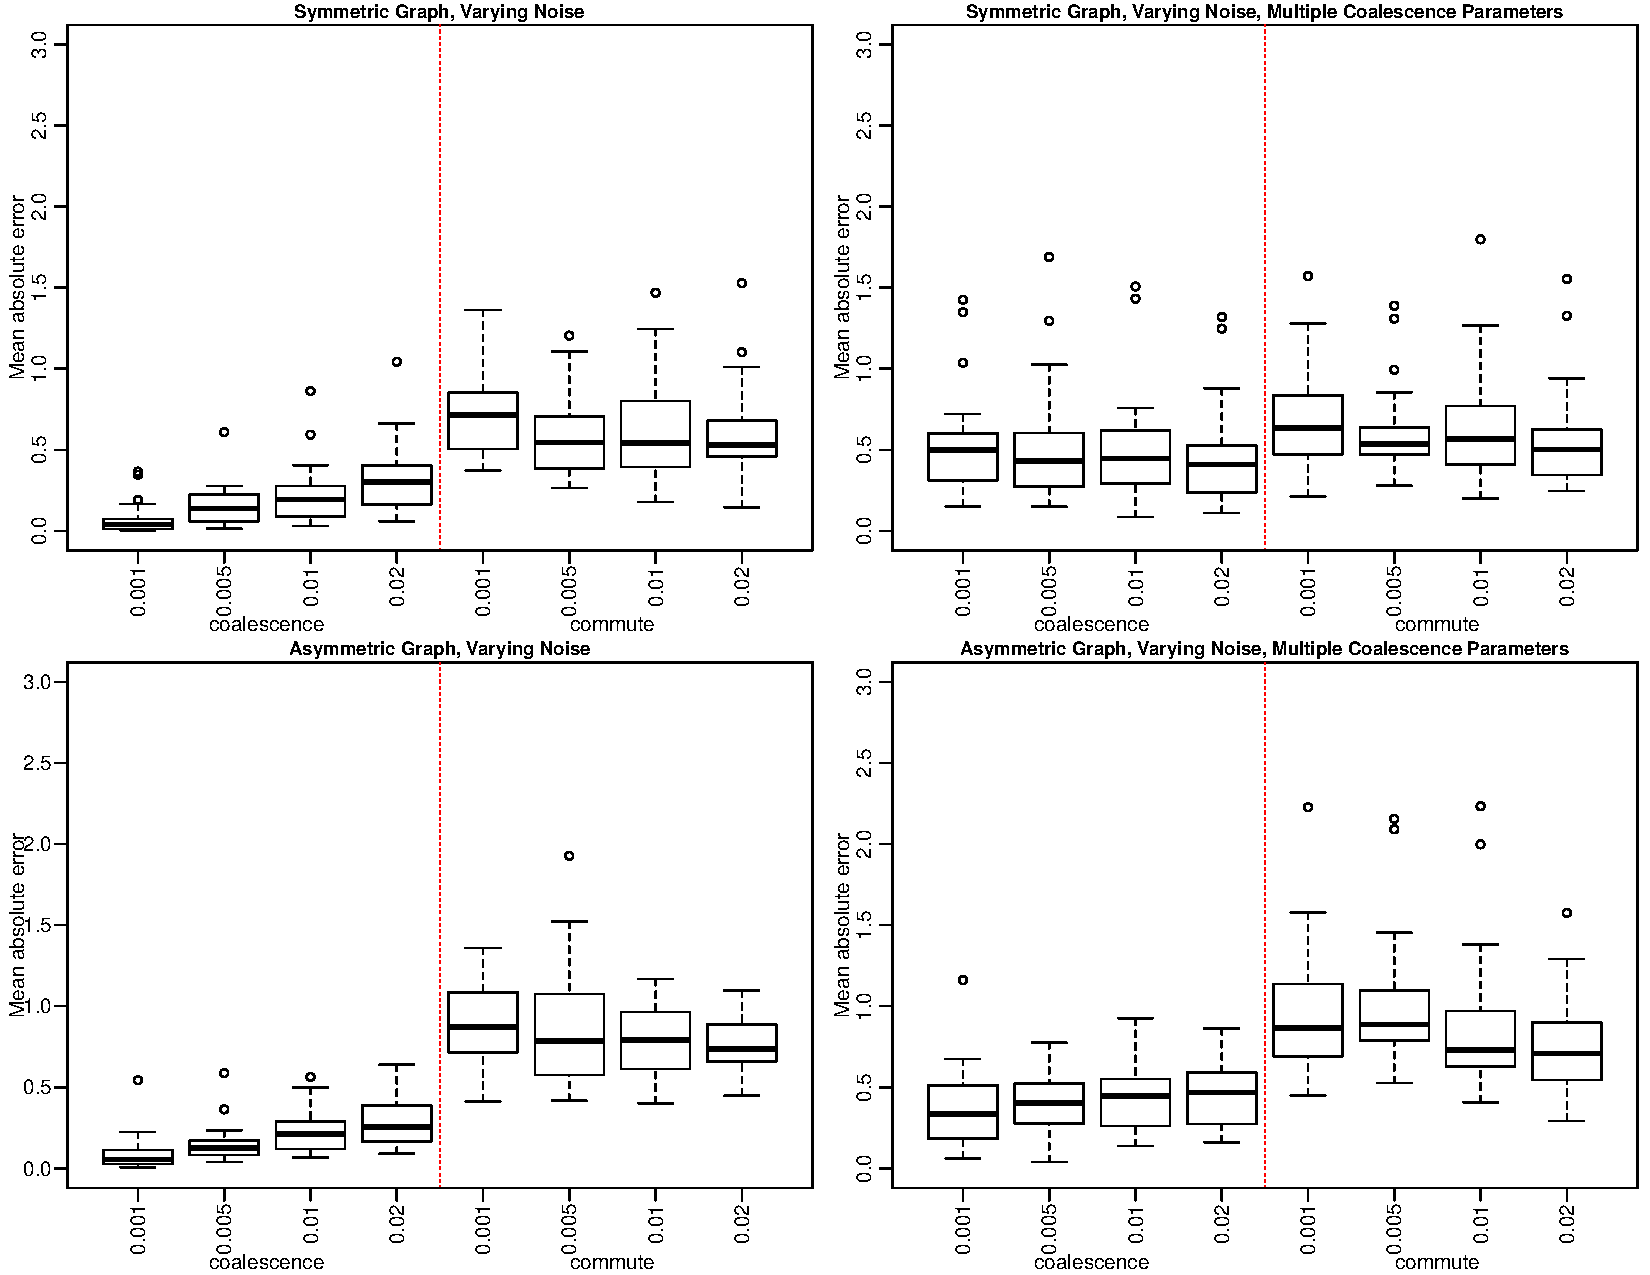
\includegraphics[scale=.6]{figs/mult_noise}
\caption{Boxplots of the mean absolute error
defined to be the absolute value difference between the true value and posterior median,
averaged across movement parameters $g$ for each of the 25 graphs in each situation.
Each box is labeled with the relative amount of noise added to $C$ to produce the values used for inference.
The top left shows the results for symmetric graphs 
when there is a single coalescence parameter for all locations,
the top right for symmetric graphs 
when there is a separate coalescence parameter for each location,
the bottom left for asymmetric graphs 
when there is a single coalescence parameter for all locations,
and the bottom right for asymmetric graphs 
when there is a separate coalescence parameter for each location.}
\label{fig:mult_noise}
\end{figure}

\begin{figure}
\centering
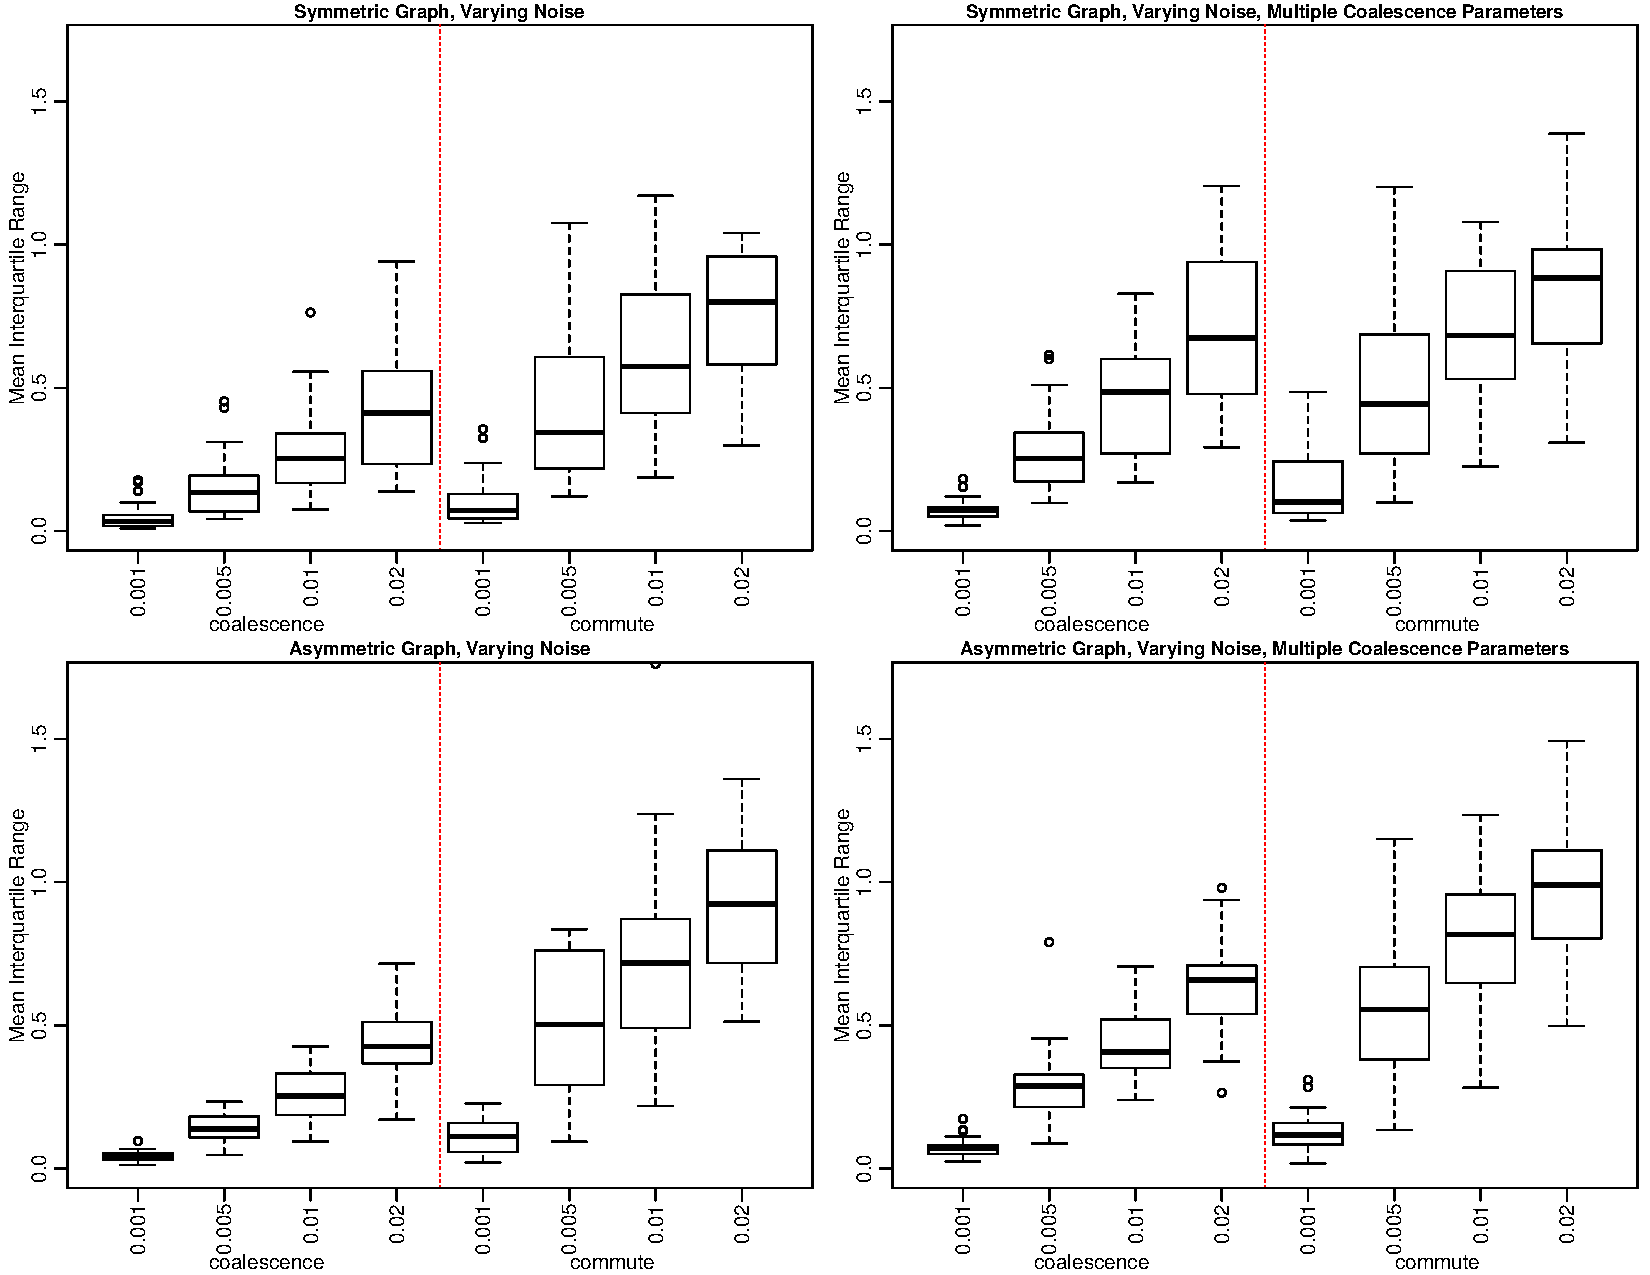
\includegraphics[scale=.6]{figs/mult_noise_iqr}
\caption{Boxplots of the mean interquartile ranges of the posterior distributions of $g$
for each of the 25 graphs in each situation.
Each box is labeled with the relative amount of noise added to $C$ to produce the values used for inference.
Subplot locations for each situation are the same as in Figure \ref{fig:mult_noise}.
%The top left shows the results for symmetric graphs 
%when there is a single coalescence parameter for all locations,
%the top right for symmetric graphs 
%when there is a separate coalescence parameter for each location,
%the bottom left for asymmetric graphs 
%when there is a single coalescence parameter for all locations,
%and the bottom right for asymmetric graphs 
%when there is a separate coalescence parameter for each location.
}
\label{fig:mult_noise_iqr}
\end{figure}


\begin{figure}
\centering
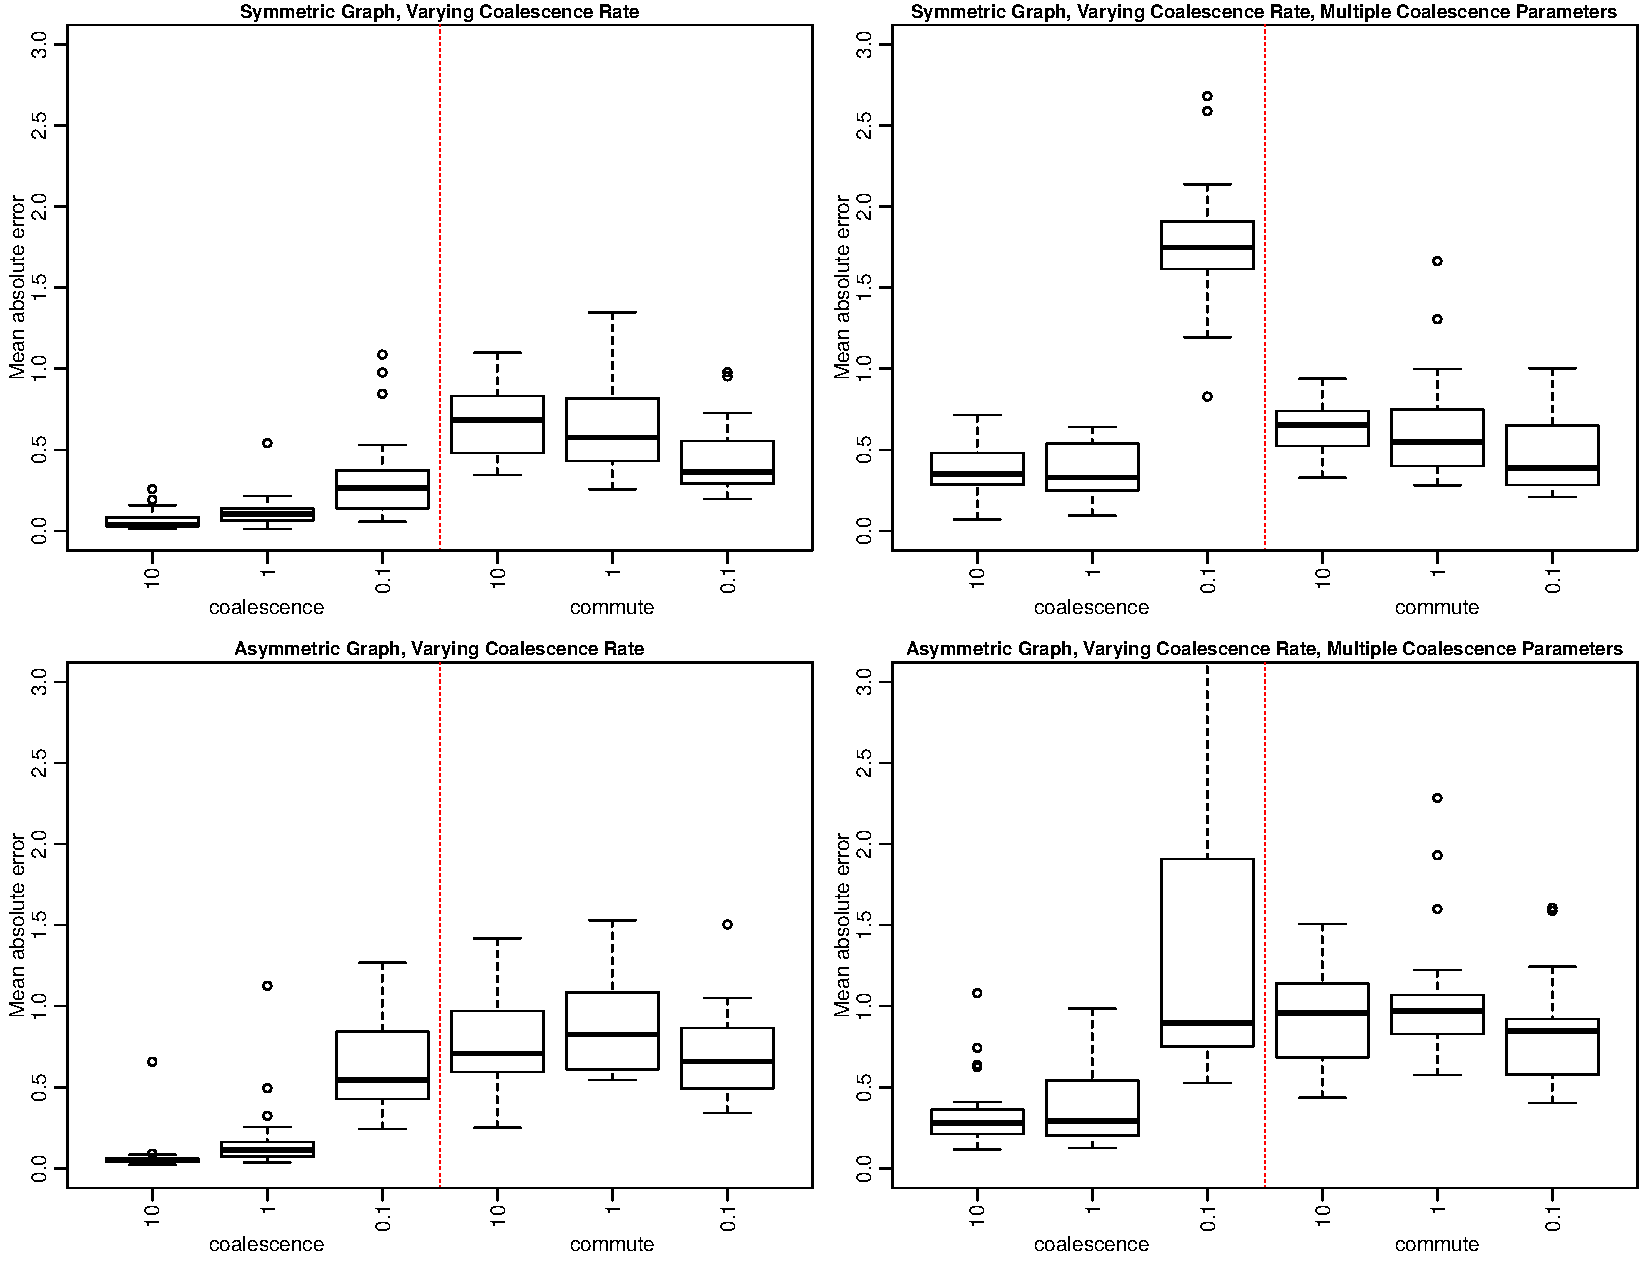
\includegraphics[scale=.6]{figs/mult_gam}
\caption{
Boxplots of the mean absolute error, %in $\hat{g}$.
defined to be the absolute value difference between the true value and posterior median,
averaged across movement parameters $g$ for each of the 25 graphs in each situation.
Each box is labeled with the coalescence rate in the underlying model for each situation.
Subplot locations for each situation are the same as in Figure \ref{fig:mult_noise}.
%The top left shows the results for symmetric graphs 
%when there is a single coalescence parameter for all locations,
%the top right for symmetric graphs 
%when there is a separate coalescence parameter for each location,
%the bottom left for asymmetric graphs 
%when there is a single coalescence parameter for all locations,
%and the bottom right for asymmetric graphs 
%when there is a separate coalescence parameter for each location.
}
\label{fig:mult_gam}
\end{figure}

\begin{figure}
\centering
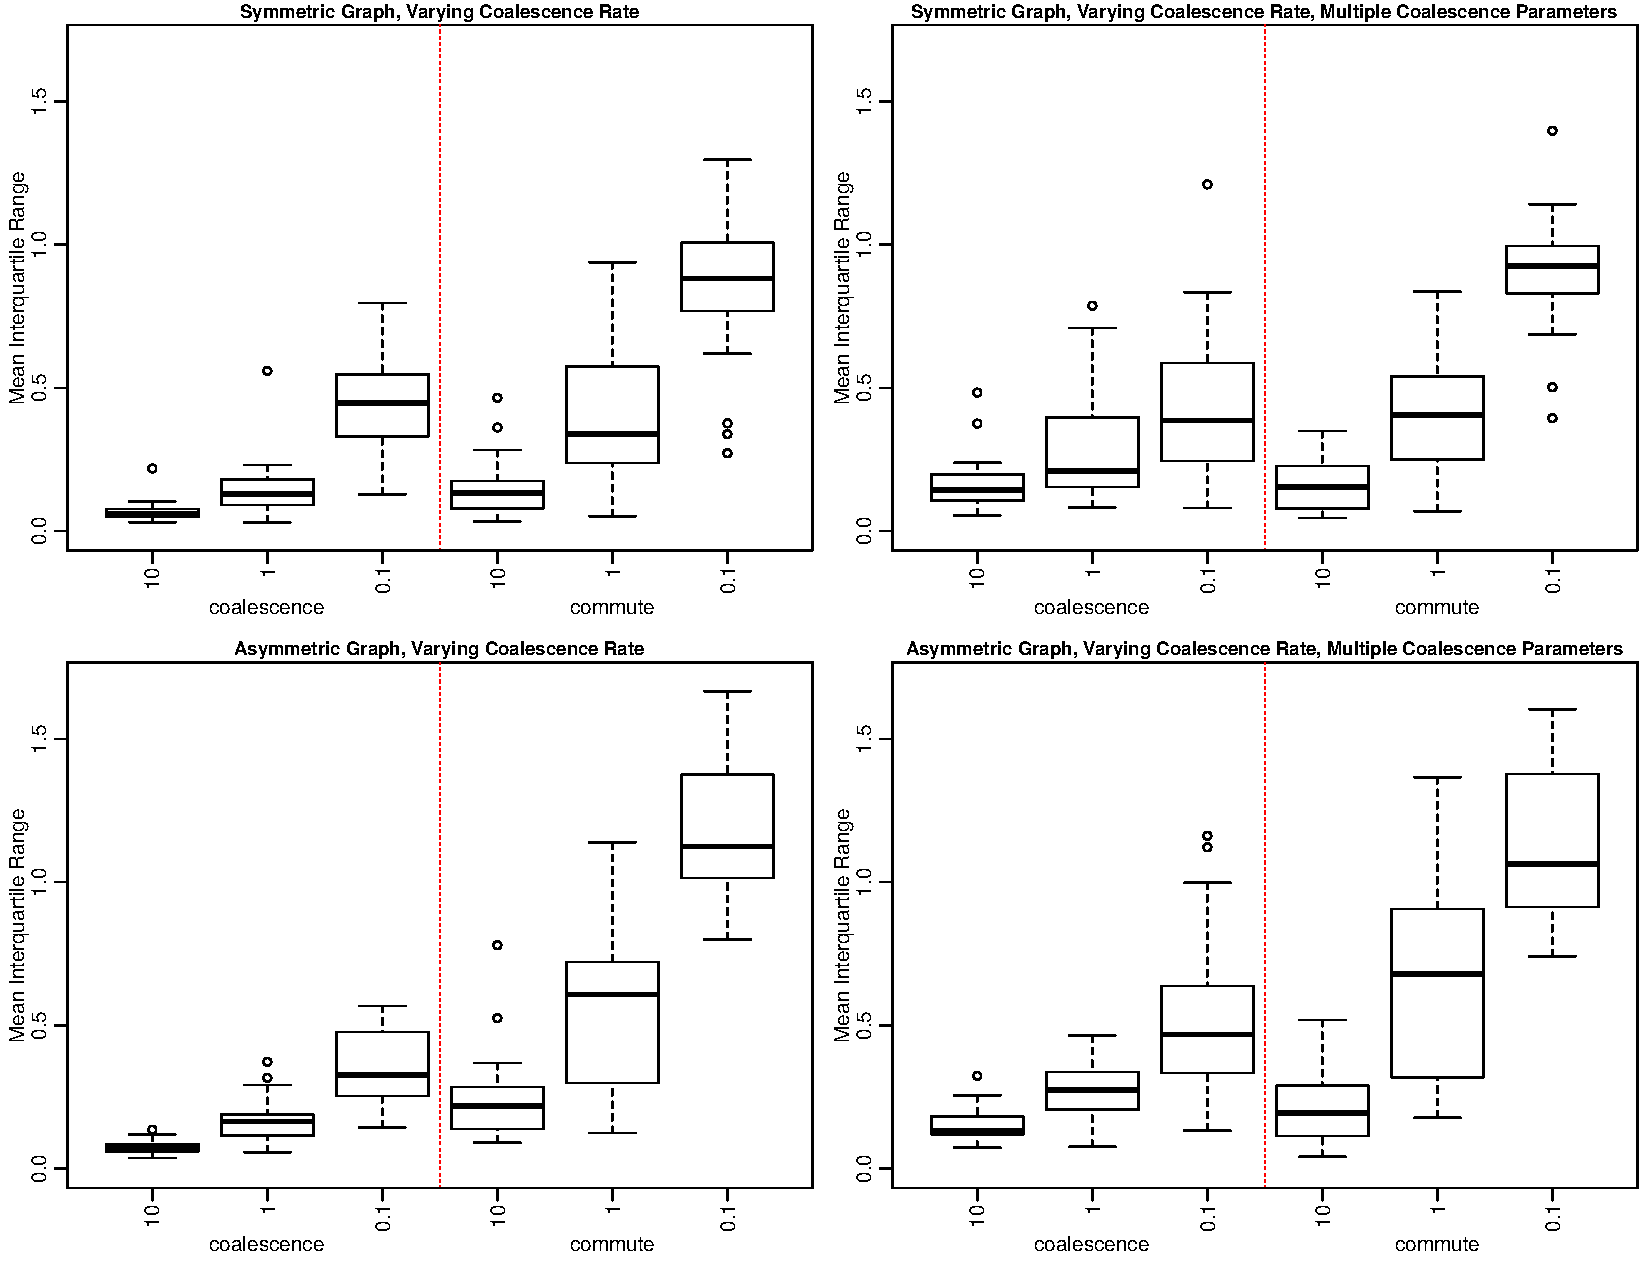
\includegraphics[scale=.6]{figs/mult_gam_iqr}
\caption{Boxplots of the mean interquartile ranges of the posterior distributions of $g$
for each of the 25 graphs in each situation.
Each box is labeled with the coalescence rate in the underlying model for each situation.
Subplot locations for each situation are the same as in Figure \ref{fig:mult_noise}.
%The top left shows the results for symmetric graphs 
%when there is a single coalescence parameter for all locations,
%the top right for symmetric graphs 
%when there is a separate coalescence parameter for each location,
%the bottom left for asymmetric graphs 
%when there is a single coalescence parameter for all locations,
%and the bottom right for asymmetric graphs 
%when there is a separate coalescence parameter for each location.
}
\label{fig:mult_gam_iqr}
\end{figure}


\begin{figure}
\centering
     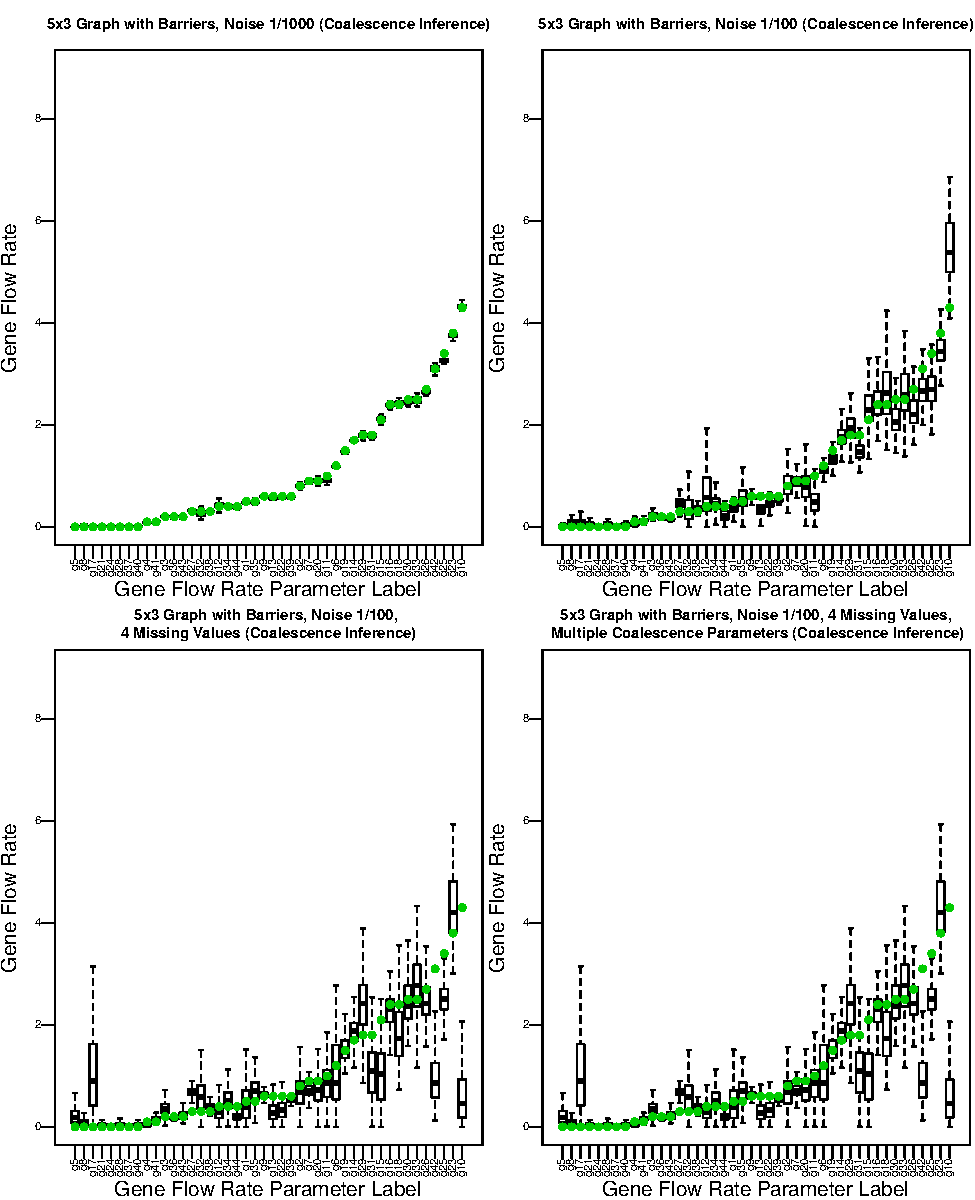
\includegraphics[scale=0.8]{figs/5x3boxplots}
    \caption{Posterior distributions for values of $g$ 
    for the 5 $\times$ 3 graph with barriers 
    for each of the analysis cases with coalescence time inference.
    See Figure \ref{fig:5x3b_grid} to see movement parameter locations.
}
    \label{fig:5x3boxplots_mult_gam}
\end{figure}


\begin{figure}
\centering
     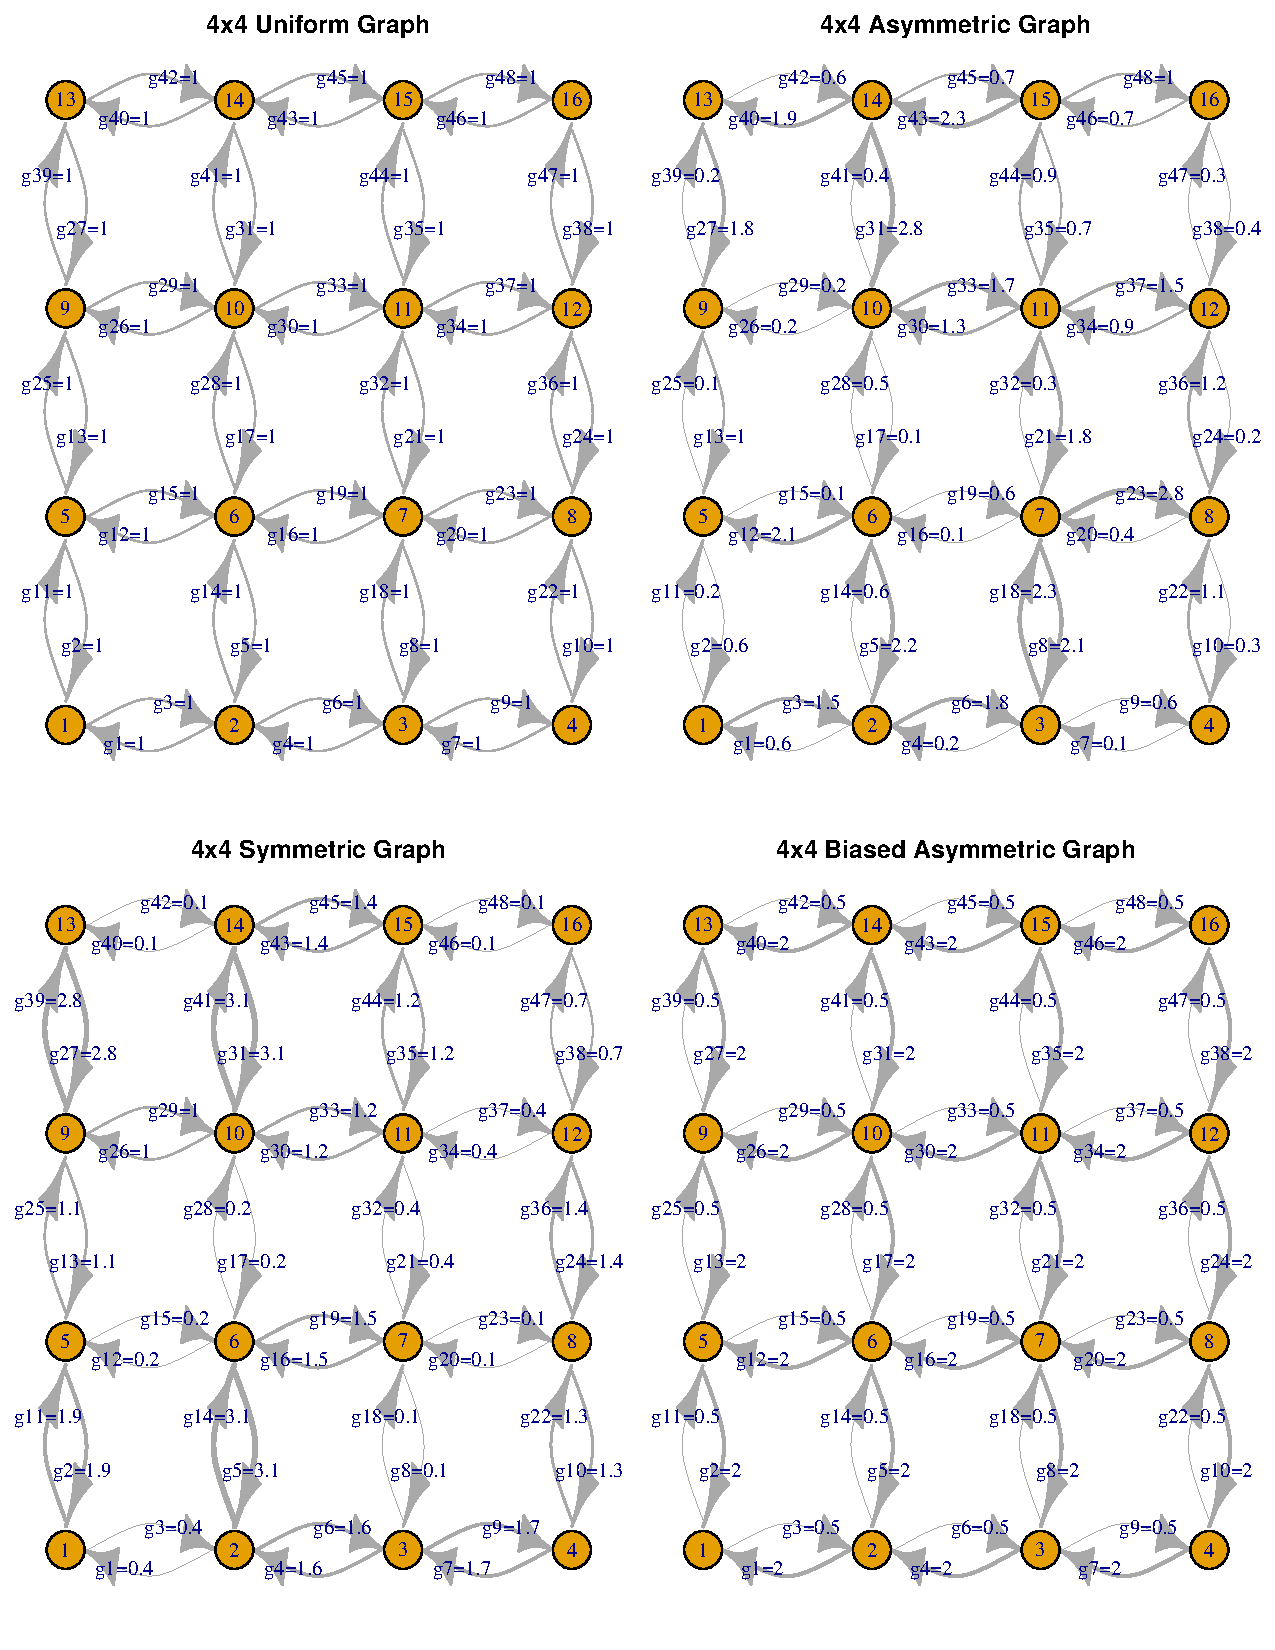
\includegraphics[scale=.7]{figs/4x4_grids}
    \caption{
        Grid structure and gene flow rates
        for the uniform graph, symmetric graph, the asymmetric graph,
        and the biased asymmetric graph 
        using the igraph R package.
    }
    \label{fig:4x4_grids}
\end{figure}


\begin{figure}
\centering
    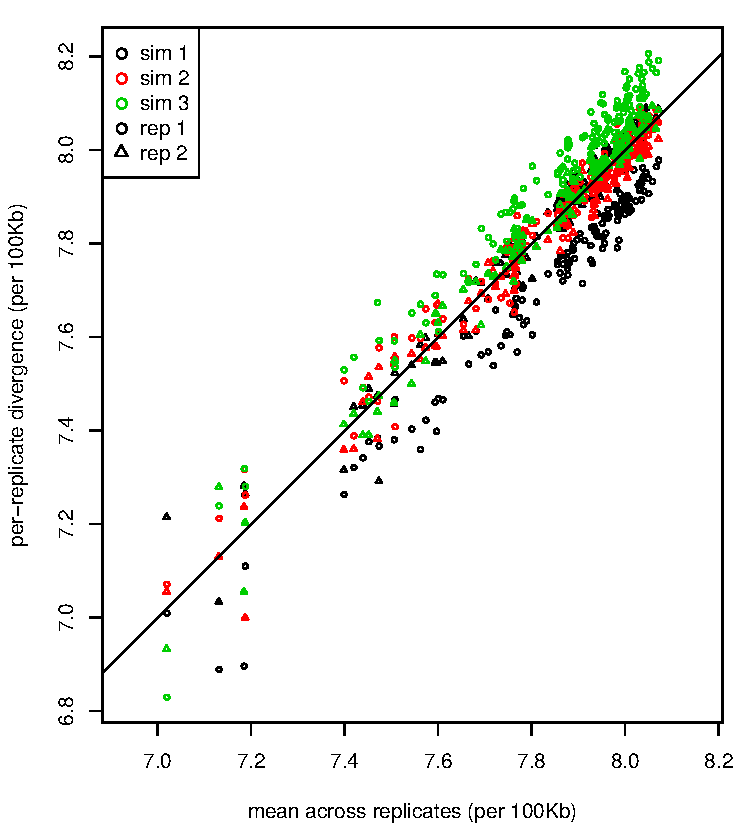
\includegraphics{{figs/all_flat_divergences.fonts}.pdf}
\caption{
    Comparison of mean coalescence times between samples and between replicates
    for a $4 \times 4$ discretization of a square landscape with uniform migration.
    Between the 16 geographic regions, there are 136 comparisons;
    these are shown for two nonoverlapping samples taken from three independent replicate simulations,
    each plotted against the mean value across all replicates.
    Colors denote simulation replicate,
    and point type (circle/triangle) denotes the sample.
    Without sampling or process noise, all points would fall on the $y=x$ line.
    Among the six sets of observations,
    simulation replicate explains 6.7\% of the variance,
    and spatial sampling explains 13.8\% of the variance.
    } \label{fig:h_val_comp}
\end{figure}

\begin{figure}
\centering
     \includegraphics{figs/example_flat_ibd}
    \caption{
        Genetic distance against geographic distance
        between all pairs of sampled individuals
        on a square landscape with uniform migration.
        Red dots denote mean genetic distances
        between sampled individuals from a $4 \times 4$ discretization of the landscape,
        as used for instance in Figure \ref{fig:more_barriers}.
        % and \textbf{(below)} biased migration.
        % The horizontal lines in the latter plot
        % are likely from comparing genomes of individuals from
        % families that have recently increased in size and geographical spread, 
        % resulting in many pairs of genomes with similar genetic distance 
        % but varying geographic distance.
    \label{fig:ibd_comp}
    }
\end{figure}

\begin{figure}
\centering
    \includegraphics[width=0.45\textwidth]{figs/bias_coal_graph}
    \includegraphics[width=0.45\textwidth]{figs/bias_commute_graph}
    \includegraphics[width=0.45\textwidth]{figs/bias_coal_dists}
    \includegraphics[width=0.45\textwidth]{figs/bias_commute_dists}
\caption{
    \textbf{(Above:)} Posterior medians and \textbf{(below)} posterior distributions
    of the inferred values of $g$ 
    for the $4 \times 4$ discretization 
    of the square landscape with biased migration,
    inferred with the
    \textbf{(left)} coalescence time-based,
    and \textbf{(right)} resistance distance-based method. 
    In the boxplots,
    black boxes show posterior distributions of gene flow rates up and to the right,
    and the adjacent green box corresponds to gene flow rate along the same edge
    in the opposite direction. 
    }
\label{fig:grid_bias_4x4_1}
\end{figure}

\begin{figure}
\centering
    \includegraphics[width=0.45\textwidth]{figs/barrier_locations}
    \includegraphics[width=0.45\textwidth]{figs/barrier_eems}
    \includegraphics[width=0.45\textwidth]{figs/barrier_coal_graph}
    \includegraphics[width=0.45\textwidth]{figs/barrier_commute_graph}
    \includegraphics[width=0.45\textwidth]{figs/barrier_coal_dists}
    \includegraphics[width=0.45\textwidth]{figs/barrier_commute_dists}
    \caption{
        Results from the \textbf{barrier} simulation:
        \textbf{(top left)} Positions of all individuals at the end of simulation.
        \textbf{(top right)} mean migration rates as estimated by EEMS.
        Below are shown
        posterior median migration rates 
            as estimated using
            \textbf{(middle left)} the coalescence time method and
            \textbf{(middle right)} the resistance distance method.
        Last are shown the posterior distributions, for
            \textbf{(bottom left)} the coalescence time method and
            \textbf{(bottom right)} the resistance distance method.
        \label{sfig:barrier_results}
    }
\end{figure}

\begin{figure}
\centering
    \includegraphics[width=0.45\textwidth]{figs/valley_locations}
    \includegraphics[width=0.45\textwidth]{figs/valley_eems}
    \includegraphics[width=0.45\textwidth]{figs/valley_coal_graph}
    \includegraphics[width=0.45\textwidth]{figs/valley_commute_graph}
    \includegraphics[width=0.45\textwidth]{figs/valley_coal_dists}
    \includegraphics[width=0.45\textwidth]{figs/valley_commute_dists}
    \caption{
        Results from the \textbf{valley} simulation:
        \textbf{(top left)} Positions of all individuals at the end of simulation.
        \textbf{(top right)} mean migration rates as estimated by EEMS.
        Below are shown
        posterior median migration rates 
            as estimated using 
            \textbf{(middle left)} the coalescence time method and
            \textbf{(middle right)} the resistance distance method.
        Last are shown the posterior distributions, for
            \textbf{(bottom left)} the coalescence time method and
            \textbf{(bottom right)} the resistance distance method.
        \label{sfig:valley_results}
    }
\end{figure}

\begin{figure}
\centering
    \includegraphics[width=0.45\textwidth]{figs/expansion_locations}
    \includegraphics[width=0.45\textwidth]{figs/expansion_eems}
    \includegraphics[width=0.45\textwidth]{figs/expansion_coal_graph}
    \includegraphics[width=0.45\textwidth]{figs/expansion_commute_graph}
    \includegraphics[width=0.45\textwidth]{figs/expansion_coal_dists}
    \includegraphics[width=0.45\textwidth]{figs/expansion_commute_dists}
    \caption{
        Results from the \textbf{expansion} simulation:
        \textbf{(top left)} Positions of all individuals at the end of simulation.
        \textbf{(top right)} mean migration rates as estimated by EEMS.
        Below are shown
        posterior median migration rates 
            as estimated using 
            \textbf{(middle left)} the coalescence time method and
            \textbf{(middle right)} the resistance distance method.
        Last are shown the posterior distributions, for
            \textbf{(bottom left)} the coalescence time method and
            \textbf{(bottom right)} the resistance distance method.
        \label{sfig:expansion_results}
    }
\end{figure}

\begin{figure}
\centering
    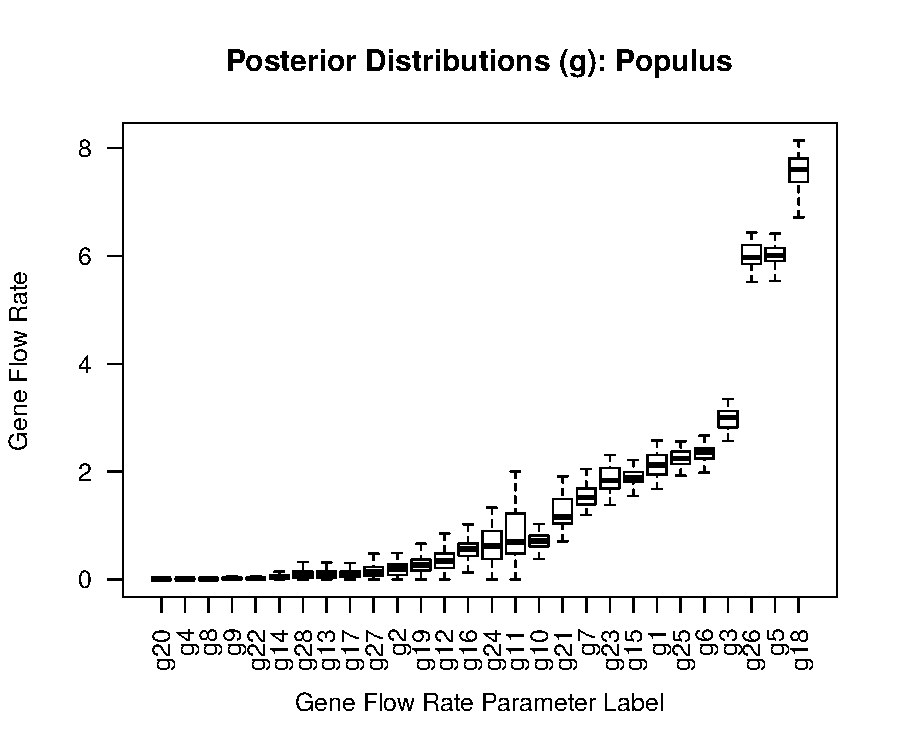
\includegraphics[width=0.7\textwidth]{poplars/posterior_dists_g_populus}
    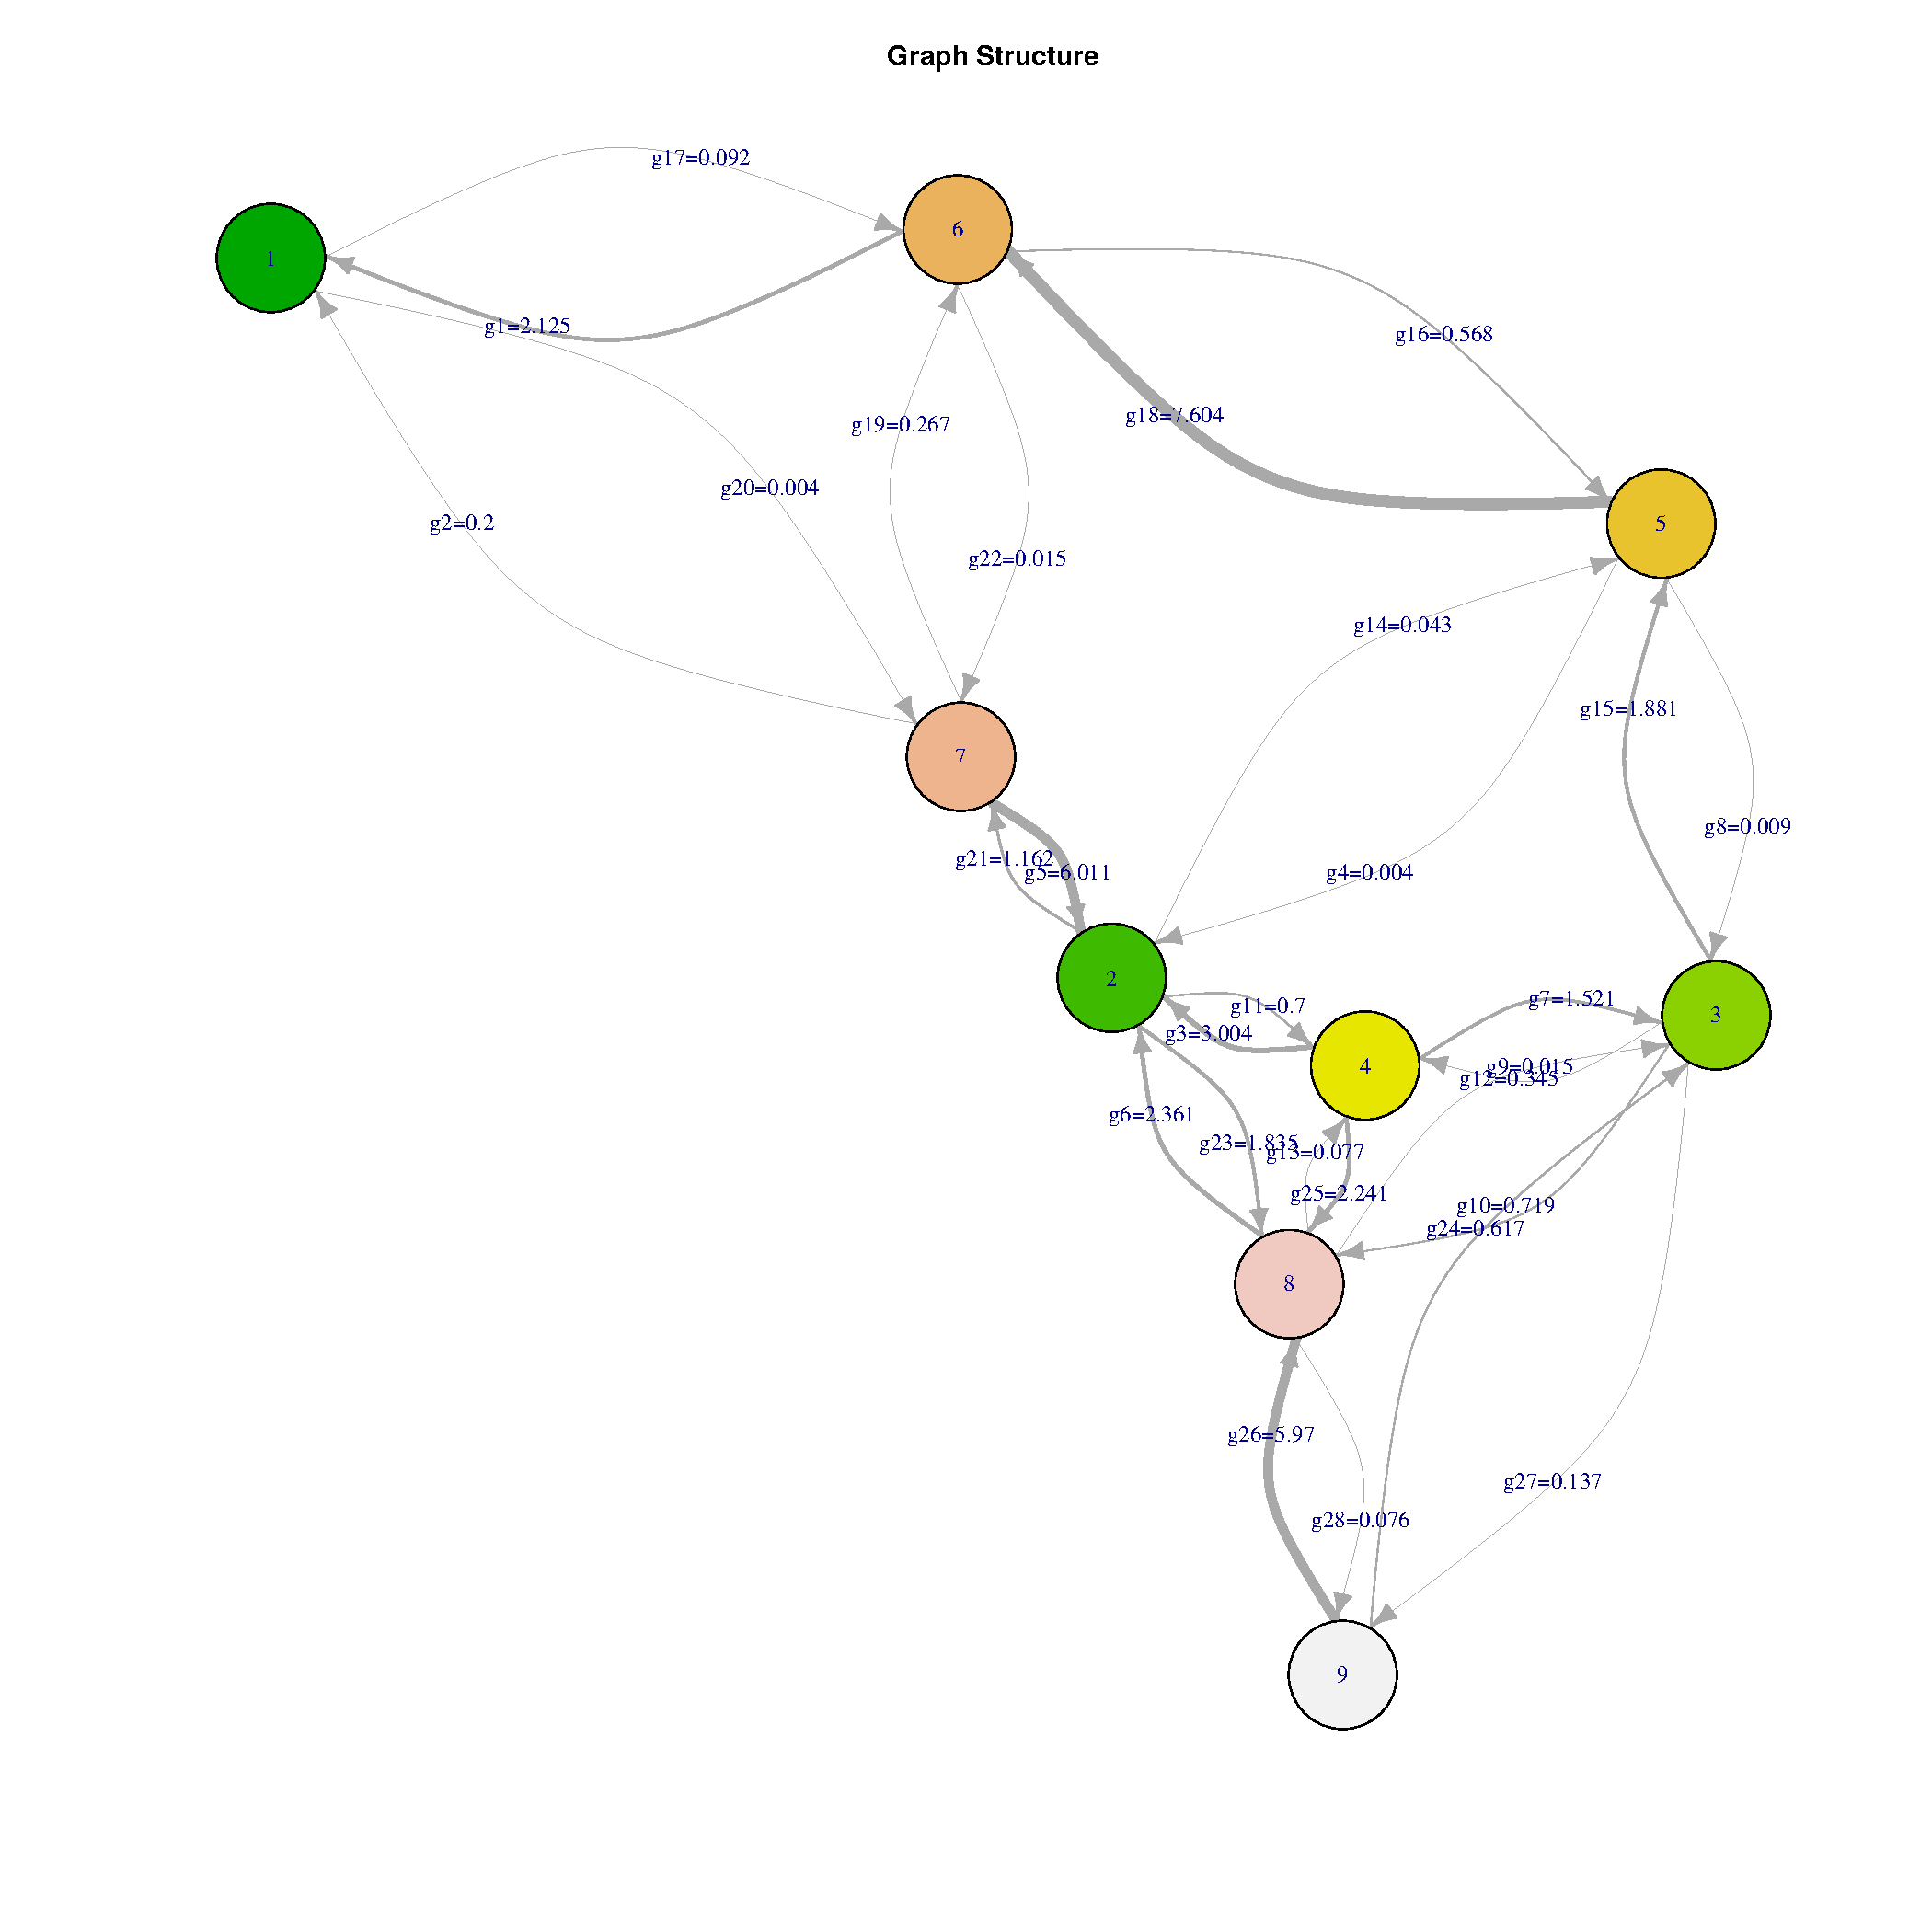
\includegraphics[width=0.7\textwidth]{poplars/grid_populus}
    \caption{
        Posterior distributions of parameters for \textit{Populus} data,
        using coalescence time inference with the model shown in Figure~\ref{fig:poplar_results}.
        \textbf{(top)} Posterior medians (dark line),
        interquartile range (box), and middle 95\% (whiskers),
        for gene flow rates.
        \textbf{(bottom)} Posterior medians, along with edge labels that match the upper figure.
        \label{sfig:poplar_g}
    }
\end{figure}

\begin{figure}
\centering
    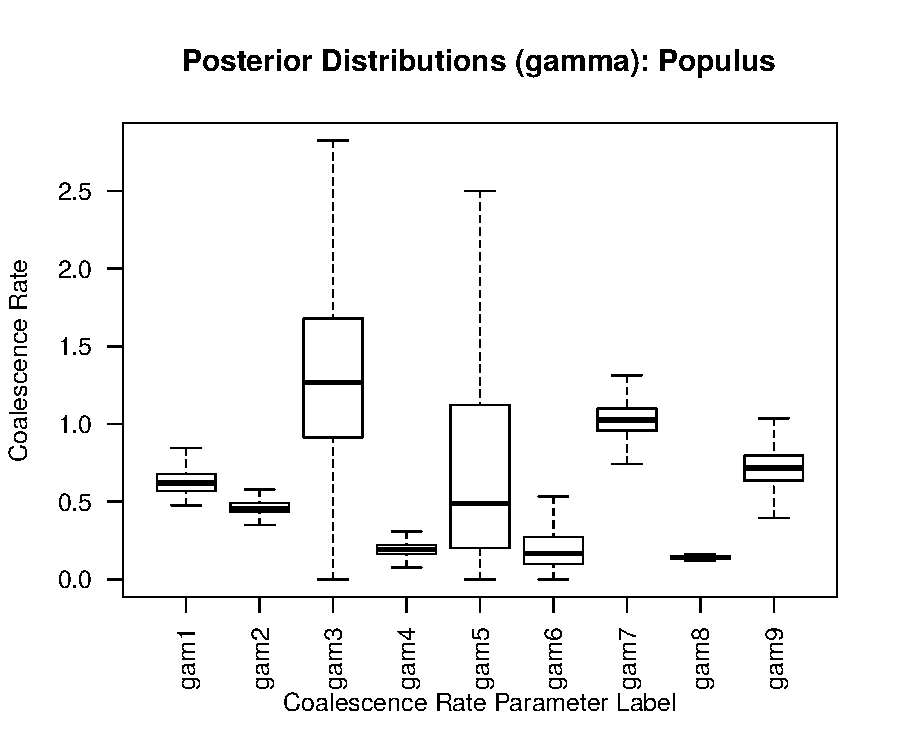
\includegraphics[width=\textwidth]{poplars/posterior_dists_gam_populus}
    \caption{
        Posterior distributions of parameters for \textit{Populus} data,
        using coalescence time inference with the model shown in Figure~\ref{fig:poplar_results}.
        Plot shows posterior medians (dark line),
        interquartile range (box), and middle 95\% (whiskers),
        for coalescence rates, labeled as in Figure~\ref{fig:poplar_results}.
        For instance, the coalescence rates for regions 4 and 8 (labeled ``gam4'' and ``gam8'')
        are inferred to be much smaller than most other regions, 
        perhaps indicating larger or older populations in southwestern British Columbia.
        \label{sfig:poplar_gam}
    }
\end{figure}

\ifsubmission
\processdelayedfloats
\fi

\newpage

\includereviews

\end{document}
